\documentclass[thesis,biblatex]{template/hust}

\addbibresource{ref.bib}
\usepackage{macros}
\usepackage{booktabs}
\usepackage{tikz}
\usetikzlibrary{shapes,arrows,positioning,fit,backgrounds,calc}

\title{基于大语言模型的课程知识命名实体识别与关系抽取}

\author{瞿明睿}
\school{计算机科学与技术学院}
\classnum{计科7班}
\stunum{U202215561}
\instructor{姚德中}
\date{2026年6月}


% 毕业论文模板
\begin{document}
    \maketitle                              % 封面
    \hypersetup{pageanchor=false}
    \thispagestyle{empty}                   % 封面后的空白页
    \null
    \clearpage
    \hypersetup{pageanchor=true}
    \authorization                          % 原创页（不保密）
    
    \pagenumbering{Roman}
    \abstractch

计算机网络课程材料包含大量非结构化知识，人工手动整理结构化文本耗时长，难以满足课程教学与研究的需要。课程文档以非结构化 PDF（Portable Document Format）与 PPT（PowerPoint）文档为主，包含大量专业术语与跨章节的复杂语义关系，不利于构建完整准确的知识图谱。实现课程知识的自动化抽取与结构化表示，对于提升教学资源的智能化利用水平具有重要意义。

为此，设计并实现一套面向计算机网络课程材料的自动化知识图谱构建系统十分必要。以大型语言模型为核心，通过提示工程方法完成课程文本的命名实体识别与关系抽取，将非结构化文档转化为结构化知识图谱，为课程教学提供可查询的知识基础。

七阶段流水线实现了从原始文档到知识图谱的端到端转换。文档预处理阶段使用多模态视觉语言模型将课程文档转换为结构化 Markdown。长文档处理采用标题层级的递归分块算法，结合词元预算控制，在保证语义连贯的前提下实现文本切分。知识抽取由实体识别和关系抽取两个子任务协同完成，分别抽取四类实体与四类关系。实体歧义通过稠密向量嵌入的规范化方法解决：利用 FAISS 向量索引与并查集算法完成实体同一性判定与等价类归并。知识融合后的三元组导入 Neo4j 图数据库，通过交互式前端界面提供关系导航与语义查询功能。

实验基于 205 份计算机网络课程 PDF 文档。原始文档经 VLM 转换为 Markdown 后，分块生成 16,438 个段落级文本块，包含多级标题内容，总计约 1,040 万词元作为知识抽取的结构化输入。在命名实体识别与关系抽取层面，启用LLM复核的最终知识图谱（\texttt{merged-fs-recheck}）包含 32,760 个实体（概念 22,696 个、机制 6,406 个、性能指标 2,192 个、协议 1,466 个）和 17,627 条关系三元组。在500条独立金标上采用"严格／软匹配／槽位／类型级"四档匹配口径评估，软匹配三元组F1为15\%~19\%，槽位F1为37\%~42\%，类型级F1可达74\%~82\%。

实验结果表明，所构建的自动化流水线能够从大规模非结构化课程材料中有效提取结构化知识，构建层次清晰、覆盖面广的知识图谱，验证了大型语言模型在课程知识建模与抽取中的可行性与有效性。

\vspace{\baselineskip}

\keywordsch 大语言模型；命名实体识别；关系抽取；知识图谱；课程知识；提示工程；实体规范化
              % 中文摘要
    \abstracten

Structuring course knowledge supports teaching and research in computer networking, yet such documents are dominated by specialized terms and cross-chapter relations, making manual knowledge graph construction costly and hard to scale. This work automates knowledge graph construction from unstructured course materials with large language models (LLMs).

A six-stage pipeline converts PDFs into Markdown, text chunks, raw triples, a merged knowledge graph, and Neo4j storage. Multimodal vision-language models perform OCR (Optical Character Recognition) and produce structured Markdown; a recursive header-aware chunking algorithm preserves document hierarchy within token limits. Chinese prompts extract four entity types (protocol, concept, mechanism, metric) and four relation types (contains, depends\_on, compared\_with, applied\_to) under zero-shot and few-shot settings, with an evidence verification gate grounding each triple in source text. Entity canonicalization combines FAISS (Facebook AI Similarity Search) with Union-Find to merge duplicates.

The pipeline processed 205 course documents and generated 16,438 chunks ($\sim$10.4 million tokens). The final knowledge graph (\texttt{merged-fs-recheck}, with LLM-based candidate review enabled) contains 32,760 entities and 17,627 relational triples. On 500 expert-reviewed gold triples, a four-tier matching protocol (Strict / Substring / Slot / Schema-level) yields triple-level F1 of 15\%--19\% under substring, 37\%--42\% under slot, and 74\%--82\% under schema-level matching. Frequent entities such as TCP, UDP, HTTP, and IP indicate that the graph captures core networking concepts, providing a structured knowledge base for networking education.

\vspace{\baselineskip}

\keywordsen Large Language Models, Named Entity Recognition, Relation Extraction, Knowledge Graph, Course Knowledge, Prompt Engineering, Entity Canonicalization
              % 英文摘要
    \tableofcontents                        % 目录
    \newpage
    \pagenumbering{arabic}
    % !TeX encoding = UTF-8
% 第1章 绪论

\section{绪\hspace{1em}论}

知识图谱是一种语义网络知识表示形式，通过结构化方式描述现实世界中的实体及其相互关系，是人工智能领域的基础信息组织形式；在教育信息化中，如何系统组织课程知识并实现智能化应用，直接影响教学质量和学习效率，而传统知识图谱的构建依赖大量人工标注，面对专业领域的命名实体识别与关系抽取任务时，标注成本高、领域适应性差、知识更新滞后等问题突出。近年来，以GPT、DeepSeek等为代表的大语言模型（Large Language Model, LLM）在自然语言理解与生成方面进步明显，为知识抽取提供了新思路：得益于大模型在零样本和少样本场景下的学习能力，即使标注数据十分有限，也能完成较高质量的信息抽取，这为教育领域知识图谱的自动化构建创造了条件。基于上述背景，本章先综述国内外基于大语言模型的命名实体识别、关系抽取与知识图谱构建的研究现状与局限，分析课程知识抽取面临的挑战并提出研究思路，最后交代论文的主要内容和组织结构。

\subsection{研究背景与意义}

\subsubsection{研究背景与趋势}

命名实体识别（Named Entity Recognition, NER）和关系抽取（Relation Extraction, RE）是信息抽取的两个核心任务，目标是从非结构化文本中自动识别预定义类型的实体并抽取实体间的语义关系。这两项技术在知识图谱构建、智能问答、文本挖掘中应用广泛\cite{ner_survey_2024,generative_ie_survey_2023}。随着深度学习的发展\cite{zhouzhihua2016}，基于神经网络的方法在标准数据集上表现良好，但这类方法通常依赖大量高质量的标注数据进行监督学习，遇到领域迁移和新实体类型时，泛化能力不足。

教育领域中，课程知识的组织专业性强，结构紧密。以计算机网络课程为例，其中涉及大量协议实体（如TCP、UDP、IP）、概念实体（如拥塞控制、流量整形）、机制实体（如三次握手、滑动窗口）以及性能指标实体（如吞吐量、时延）。这些实体之间存在复杂的依赖和应用关系，是课程知识体系的核心。教育领域的知识抽取面临独特的挑战：专业术语存在歧义、知识表达方式多样、对证据可追溯性有要求，传统的有监督学习方法难以直接适应。

大语言模型的兴起为解决上述难题提供了新思路。近年的综述研究表明，大语言模型已从预训练语言模型发展为覆盖训练优化、能力评测和行业应用的通用技术体系\cite{wangyaozu2024_llm_survey}。通过提示工程（Prompt Engineering）和上下文学习（In-Context Learning），大语言模型可以在仅给定少量示例甚至无示例的情况下完成特定任务\cite{llms_kg_survey_2023}，这对标注数据稀缺的教育领域尤其重要。大模型较强的语义理解能力使其能捕捉文本中隐含的语义关系，涌现能力则有助于识别传统方法难以发现的隐性知识关联，而预训练阶段积累的知识表示也使其能更好地理解领域专业知识。

\subsubsection{课题目的与意义}

本课题研究利用大语言模型进行课程知识的命名实体识别与关系抽取，构建面向计算机网络课程的知识图谱自动化构建系统。具体包含以下目标：

探索适用于教育领域的大模型提示策略。通过设计任务特定的提示模板，结合零样本和少样本学习方式，提升大模型在课程知识抽取任务上的表现。针对不同的实体类型和关系类型，设计差异化的提示策略，利用大模型的上下文学习能力。通过实验对比，确定提示设计原则和参数配置。研究不同提示元素（如任务描述、示例、输出格式说明）对抽取性能的影响，为提示工程提供实践参考。

建立知识抽取的质量保障机制。引入证据验证和一致性检查机制，降低大模型生成错误知识的风险，保障知识图谱的准确性。设计自动化的质量评估指标，对抽取结果进行实时监控和反馈。建立人机协作的审核流程，兼顾效率与质量。开发冲突检测算法，识别并解决知识抽取中的逻辑矛盾和不一致问题。

设计知识图谱构建流水线。将文档解析、文本预处理、实体识别、关系抽取、知识融合等环节整合为统一流程，形成可复用的教育知识图谱构建方案。设计模块化架构，支持灵活的配置和扩展，以适应不同学科的知识抽取需求。实现从原始PDF到结构化知识图谱的端到端自动化。提供清晰的配置接口和日志监控，降低系统的使用门槛。

本课题在理论和应用两个层面均具有价值。理论上，探索大模型在专业领域知识抽取中的应用模式，为领域自适应的信息抽取方法研究提供参考。研究成果有助于理解大语言模型在特定领域的表现特征，为提示工程和领域适配方法的发展提供实证依据。通过实验设计和结果分析，探讨大模型在教育知识抽取任务中的能力边界和优化方向，为少样本和零样本场景下的信息抽取方法研究提供参考。

应用上，研究成果可直接用于课程资源的智能化管理和个性化学习推荐。构建的知识图谱可应用于智能问答、学习路径推荐、知识点关联分析等教育场景，改善教学效果和学习体验。教师可借助知识图谱快速定位课程重点，设计更有针对性的教学内容；学生可通过知识图谱建立不同知识点之间的关联，形成完整的知识体系。研究成果还可推广至其他专业领域的知识图谱构建。

\subsection{国内外研究现状}

\subsubsection{基于大模型的命名实体识别}

近年来，利用大语言模型进行命名实体识别的方法发展迅速，研究者围绕提示设计、输出约束、数据增强等方向做了大量工作。

GPT-NER\cite{gpt_ner_2023}提出了一种基于特殊标记的提示转换方法，引入\texttt{@@\#\#}等标记符号，将NER任务转化为大模型易于理解的文本生成任务，并配合自验证机制提高识别准确率。该方法解决了大模型在结构化预测任务上的格式遵循问题，使模型输出可直接解析为结构化标注。实验表明，该方法在多个标准数据集上取得了与监督学习方法相当甚至更优的成绩。研究还探索了不同标记符设计对模型性能的影响，发现特定的分隔符组合能提升实体边界识别的准确性。通过自一致性检查，降低了格式错误的发生率。

SLIMER\cite{slimer_2024}针对少样本NER场景，提出了基于实体类型定义和标注指南的提示设计框架。该方法为每种实体类型提供详细的定义描述和标注规范，引导大模型更好地理解任务要求，在跨领域NER任务上效果好。研究还发现，为实体类型添加具体示例和边界案例，能提升模型的识别准确率。通过负例说明，帮助模型理解哪些文本片段不应被识别为特定类型的实体，降低了误识别率。该方法的核心思路是利用人类标注知识指导模型学习，即使没有大量标注数据也能取得较好效果。

CodeIE\cite{codeie_2023}探索了将Python代码作为提示的新范式，利用代码的结构化特性引导大模型生成结构化的NER输出。研究表明，相比自然语言提示，代码风格的提示在结构化预测任务上具有明显优势，因为代码的语法约束能更好地引导模型生成符合格式要求的输出。该方法在零样本和少样本设置下均表现出较好的泛化能力，能够适应新的实体类型而不需要重新训练模型。代码表示还方便集成复杂的约束规则和验证逻辑，提升了抽取质量。

LLM-DA\cite{llm_da_2024}聚焦数据增强方向，提出了基于大模型的上下文级和实体级数据增强方法。通过在上下文层面进行语义变换、在实体层面进行同义词替换和边界扰动，扩充了训练数据的多样性。该方法对缓解少样本场景下的数据稀缺问题有重要参考意义，能提升模型的鲁棒性和泛化能力。研究还提出了基于大模型的数据质量评估方法，自动筛选高质量的增强样本。通过迭代增强策略逐步扩充训练数据集，在保持数据质量的同时扩大数据规模。

\subsubsection{基于大模型的关系抽取}

在关系抽取领域，大语言模型同样展现了潜力，研究者在示例选择、推理机制、任务分解等方面做了大量工作。

GPT-RE\cite{gpt_re_2023}提出了一种任务感知的示例检索策略，根据输入文本与候选示例的语义相似度动态选择上下文示例，提升了少样本关系抽取的性能。该方法通过引入实体感知的示例编码机制，使模型能更好地理解与当前任务相关的上下文信息，从而在复杂的关系分类任务中取得更好效果。实验结果表明，合理的示例选择策略对最终性能的影响甚至超过了模型规模的选择。研究还探索了动态示例库更新机制，使系统能够随着运行不断积累高质量的示例。

Revisiting-RE\cite{revisiting_re_2023}分析了链式思维（Chain-of-Thought, CoT）推理在关系抽取任务中的作用，发现显式引导大模型进行逐步推理能提高复杂关系的识别准确率，在涉及多跳推理的场景中尤为明显。研究还探讨了不同推理路径设计对最终性能的影响，可供提示工程设计参考。研究发现，关系特定的推理模板比通用模板能取得更好的效果，将复杂的关系判断分解为多个简单的推理步骤，可降低模型的判断难度。

AutoRE\cite{auto_re_2024}提出了一种基于关系-头实体-事实（Relation-Head-Fact）分解的抽取范式，将复杂的关系抽取任务分解为多个子任务，降低了模型的生成难度。该方法结合了基于人类反馈的强化学习（Reinforcement Learning from Human Feedback, RLHF）训练范式，使模型输出更契合知识图谱的结构要求。实验结果表明，分解策略能减少关系抽取中的错误传播，提升端到端的抽取质量。该方法的优势在于模块化设计，每个子任务可独立优化和评估。

\subsubsection{统一信息抽取与知识图谱构建}

统一信息抽取框架旨在通过单一模型同时完成实体识别、关系抽取等多项任务，以提升系统的效率和一致性。

InstructUIE\cite{instructuie_2023}提出了基于指令微调的多任务信息抽取框架，通过设计统一的指令格式将不同类型的信息抽取任务转化为一致的文本到文本生成问题，实现了跨任务的知识迁移。该方法在多个信息抽取任务上取得了有竞争力的性能，显示了统一框架在多任务上的优势。研究还发布了大规模的多任务指令数据集，为后续研究提供了数据基础。通过统一编码，模型能够学习不同任务之间的共享知识，提升泛化能力。

GoLLIE\cite{gollie_2023}延续了代码作为提示的思路，将标注指南编码为Python类型定义和约束条件，利用大模型的代码理解能力进行结构化信息抽取。该方法在零样本场景下表现出较好的泛化能力，能够适应新的实体类型和关系类型而不需要重新训练。代码形式的约束条件使模型能更准确地理解抽取任务的边界和要求，同时方便集成复杂的业务规则。该方法的优势在于可解释性强，便于调试和验证。

OneKE\cite{oneke_2025}提出了一种多智能体协作的知识抽取架构，通过调度多个专门化的抽取智能体分别负责实体识别、关系分类、属性抽取等子任务，再由融合模块整合各智能体的输出，提升了抽取质量。该架构的优势在于能发挥不同智能体的专长，通过协作机制取得比单一模型更好的抽取效果。系统还引入了置信度加权机制，在融合过程中优先采纳高置信度的预测结果。智能体之间的通信协议设计是该系统的主要创新。

在教育领域知识图谱构建方面，Educational-KG-Pipeline\cite{educational_kg_pipeline_2025}提出了一套面向教育资源的五阶段知识图谱构建流水线，涵盖数据采集、预处理、知识抽取、知识融合和图谱存储等环节，为教育领域的知识图谱构建提供了参考方案。Graphusion\cite{graphusion_2024}则专注于零样本知识图谱构建，提出了基于多源知识融合的图谱扩展方法，能够在无标注数据的情况下实现知识图谱的自动构建和扩展。

\subsubsection{教育领域知识图谱}

教育领域知识图谱研究近年来进展较快，研究者探索了多种构建和应用方法。

LLM-Curriculum-KG\cite{llm_curriculum_kg_2025}探索了人机协作的课程知识建模方法，将大模型的自动抽取能力与领域专家的知识校验相结合，实现了课程知识体系的构建。该方法采用人在回路（Human-in-the-Loop）模式，在保证知识准确性的同时提升了构建效率。研究还提出了面向课程知识的专门化实体类型体系和关系模式，为教育领域的知识表示提供了参考。实验结果表明，人机协作模式相比纯自动或纯人工的方式，在效率和质量间取得了平衡。

LLMs-KG-Survey\cite{llms_kg_survey_2023}对基于大语言模型的知识图谱技术进行了综述，分析了提示工程、指令微调、检索增强生成等技术在知识抽取、知识补全、知识推理等任务中的应用，梳理了当前研究的主要挑战和发展方向。综述强调领域适应性和知识质量控制在实践中的重要性，还建立了一套评估框架，用于比较不同方法在知识准确性、覆盖率和一致性等方面的表现。

\subsubsection{现有工作的局限与本课题切入点}

综上，基于大语言模型的信息抽取技术发展迅速，但在面向教育领域的课程知识抽取方面，仍有研究空白。现有工作在方法层面各有侧重：GPT-NER和SLIMER关注NER的提示设计，GPT-RE和AutoRE关注RE的任务分解，InstructUIE和GoLLIE关注统一信息抽取框架，但较少有工作将NER、RE与端到端的知识图谱构建流水线在课程知识场景下进行系统整合。在教育领域，LLM-Curriculum-KG和Educational-KG-Pipeline分别从人机协作和流水线构建的角度进行了探索，但在知识质量的可验证性、面向课程材料的专业化Schema设计以及零样本/少样本提示策略的系统对比方面仍需进一步研究。

针对上述空白，聚焦三个关键问题：一是如何设计面向课程知识的多层次实体与关系Schema，并进行零样本和少样本提示策略的系统对比；二是如何通过证据门控机制保障抽取知识的可验证性和可追溯性；三是如何构建模块化、可扩展的端到端知识图谱构建流水线。相关技术方案将在第三章和第四章中详细阐述。

\subsection{面临的挑战与研究思路}

\subsubsection{课程知识抽取面临的挑战}

尽管大语言模型在通用自然语言处理任务上表现优异，但在面向课程知识的信息抽取任务中，仍然面临以下挑战：

一是领域适应性不足。通用大语言模型知识面广，但对特定领域的专业术语和知识体系理解有限。课程知识涉及大量领域特定的概念和关系类型，需要针对教育场景进行专门的模型适配和提示设计。不同学科的知识表达方式不同，如何设计通用的领域适配框架仍是一个需要解决的问题。计算机网络这类课程专业性较强，涉及大量协议规范和技术细节，需要模型具备较强的领域理解能力。例如，同一术语在不同上下文中可能指代不同的概念，模型需要结合上下文才能准确理解。

二是输出结构化困难。大语言模型的输出本质上是自由文本，而知识图谱构建需要严格结构化的三元组数据。如何设计有效的提示策略和输出约束机制，确保模型生成的表示符合规范，是实际应用中的关键问题。在处理复杂的嵌套实体和多关系场景时，结构化的准确性直接影响后续知识融合的效果。输出中的格式错误、实体边界识别偏差、关系类型混淆等问题都会降低最终知识图谱的质量。如何设计可解析的输出格式，并处理模型偶尔产生的格式偏离，也需要在工程实现中解决。

三是知识准确性难以验证。大语言模型存在幻觉（Hallucination）现象，可能生成表面合理但实际错误的信息。在教育场景中，知识准确性尤其重要，需要建立证据验证机制，确保抽取结果的可信度和可追溯性。如何量化模型输出的置信度，在置信度偏低时触发人工审核，也是实际部署中需要权衡的问题。对于关键的专业知识点，抽取错误可能对学习者产生误导，因此需要质量控制。将抽取的知识与原文片段关联建立证据溯源，有助于提升可信度。

四是规模化处理复杂。课程材料通常以PDF、PPT等多种形式存在，包含大量图文混排内容。如何构建端到端的自动化处理流水线，将原始文档高效转换为结构化知识，是工程实现层面的主要挑战。大规模文档处理时的计算效率和成本控制也是实际应用中需要考量的因素。对于包含复杂排版、数学公式和图表说明的技术文档，准确提取其中的知识内容存在较大技术难度。如何设计可扩展的架构以支持持续的知识更新和增量处理，也是长期运营中的问题。

\subsubsection{挑战到方案的映射}

针对上述四个方面的挑战，设计了一套系统的技术方案，从领域适配、输出规整、质量保障和工程架构四个维度进行应对，如图\ref{fig:1-1}所示。

\begin{figure}[ht]
    \centering
    \begin{tikzpicture}[
        node distance=0.6cm and 0.5cm,
        challenge/.style={
            rectangle, rounded corners=2pt, draw=black!70, dashed, fill=black!4,
            text width=2.8cm, minimum height=1cm, align=flush center,
            font=\footnotesize, text=black!85, inner xsep=4pt
        },
        solution/.style={
            rectangle, rounded corners=2pt, draw=black!70, fill=black!8,
            text width=2.8cm, minimum height=1cm, align=flush center,
            font=\footnotesize, text=black!85, inner xsep=4pt
        },
        center/.style={
            rectangle, rounded corners=4pt, draw=black, very thick, fill=black!15,
            text width=2.4cm, minimum height=1.2cm, align=center,
            font=\small\bfseries, text=black!90, inner xsep=4pt
        },
        arr_l/.style={-{stealth}, thick, draw=black!70},
        arr_r/.style={-{stealth}, thick, draw=black!70}
    ]
    % Left: Challenges
    \node[challenge] (c1) {领域适应性不足\\{\scriptsize 专业术语理解有限，领域特征表达多样}};
    \node[challenge, below=0.2cm of c1] (c2) {输出结构化困难\\{\scriptsize 自由文本与结构化三元组的需求矛盾}};
    \node[challenge, below=0.2cm of c2] (c3) {知识准确性难以验证\\{\scriptsize 大模型幻觉问题，教育场景可信度要求高}};
    \node[challenge, below=0.2cm of c3] (c4) {规模化处理复杂\\{\scriptsize PDF/PPT等多源文档的端到端自动化挑战}};

    % Center
    \node[center, right=1.0cm of c2] (sys) {课程知识\\[0.1cm]抽取系统};

    % Right: Solutions
    \node[solution, right=1.0cm of sys] (s1) {领域Schema与提示策略（第三章）\\{\scriptsize 四类实体与关系体系，零/少样本设计}};
    \node[solution, below=0.2cm of s1] (s2) {两阶段抽取架构（第三章）\\{\scriptsize Propose-Review流程，JSON结构化约束}};
    \node[solution, below=0.2cm of s2] (s3) {证据门控机制（第三章）\\{\scriptsize 原文子串匹配验证，可追溯的证据溯源}};
    \node[solution, below=0.2cm of s3] (s4) {六阶段流水线架构（第四章）\\{\scriptsize 模块化设计，断点续跑，独立扩展}};

    % Arrows: challenges → center (fan pattern, all converge on sys.west)
    \draw[arr_l] (c1.east) -- (sys.west);
    \draw[arr_l] (c2.east) -- (sys.west);
    \draw[arr_l] (c3.east) -- (sys.west);
    \draw[arr_l] (c4.east) -- (sys.west);

    % Arrows: center → solutions (fan pattern, all diverge from sys.east)
    \draw[arr_r] (sys.east) -- (s1.west);
    \draw[arr_r] (sys.east) -- (s2.west);
    \draw[arr_r] (sys.east) -- (s3.west);
    \draw[arr_r] (sys.east) -- (s4.west);

    % Labels (consistent 0.2cm spacing)
    \node[below=0.2cm of c4, font=\footnotesize, text=black!60] (clabel) {面临挑战};
    \node[below=0.2cm of s4, font=\footnotesize, text=black!60] (slabel) {解决思路};
    \end{tikzpicture}
    \caption{课程知识抽取面临的挑战与解决思路}\label{fig:1-1}
\end{figure}

具体而言：针对领域适应性不足，定义了覆盖协议、概念、机制和性能指标的四类实体类型体系，以及包含、依赖、对比和应用于的四类关系类型体系，结合零样本和少样本两种提示策略提升LLM的领域理解能力；针对输出结构化困难，设计了Propose-Review两阶段抽取架构，通过审核阶段的类型合法性检查、证据子串匹配和实体存在性验证等多项约束，将LLM的自由文本输出规整为结构化三元组；针对知识准确性难以验证，提出了证据门控机制，要求每条三元组必须附带原始文本块的连续原文子串作为依据，实现了输出结果的自动验证与可追溯；针对规模化处理复杂，构建了文档渲染、OCR文字提取、文本分块、知识抽取、知识融合和图数据库导入的六阶段端到端流水线，各阶段以文件系统中间产物解耦，支持独立扩展与断点续跑。这些技术方案的详细设计将在第三章和第四章中展开。

\subsection{论文的主要内容与结构}

\subsubsection{论文主要内容}

本课题围绕基于大语言模型的课程知识命名实体识别与关系抽取展开研究，构建了面向计算机网络课程的知识图谱自动化构建系统。主要研究内容包括：

\textbf{（1）多源课程语料库构建}

构建了包含205份PDF文档的多源课程语料库，涵盖教材、课件、实验指导、RFC文档等多种类型。设计了标准化的文档预处理流程，实现从PDF到结构化文本的自动转换，最终生成16,438个文本块，总计约1,040万词元（tokens），为后续的知识抽取提供了数据基础。针对不同来源的文档特性，设计了差异化的解析策略，保障文本提取的完整性和准确性。对于包含复杂排版的技术文档，采用了专门的处理方法以保留知识结构信息。建立了文档元数据管理系统，记录每份文档的来源、类型和处理状态。

\textbf{（2）基于大模型的命名实体识别}

针对课程知识的特性，定义了协议、概念、机制、性能指标四类实体类型。设计了零样本和少样本两种提示策略，通过任务特定的提示模板引导大模型识别文本中的命名实体。实验表明，该方法在没有大规模标注数据的情况下依然能达到较高的识别准确率。针对不同实体类型的特点，设计了差异化的提示模板和示例选择策略，提升了识别效果。引入了实体链接机制，将识别出的实体与标准化术语库关联，解决了实体歧义和同义词问题。

\textbf{（3）基于大模型的关系抽取}

定义了包含、依赖、对比、应用于四类关系类型。提出了“提议-审核”两阶段抽取策略，第一阶段由大模型生成候选关系三元组，第二阶段通过证据验证机制确保抽取结果的准确性和可追溯性。引入了关系约束规则，对不符合逻辑的关系进行过滤，降低了错误率。设计了关系置信度评估机制，为后续的知识融合提供质量依据。对于复杂的多跳关系，设计了迭代抽取策略，逐步构建关系链。建立了关系类型层次结构，支持细粒度的关系分类。

\textbf{（4）知识抽取流水线设计}

设计了涵盖文档解析、图像转换、文本识别、文本分块、知识抽取、知识融合、图谱导入七个环节的自动化处理流水线。各模块之间通过标准化接口进行数据交换，支持灵活的配置和扩展。实现了基于配置文件的流水线编排，用户可根据需求自定义处理流程和参数设置。流水线支持断点续处理和增量更新，提高了大规模数据处理的效率。提供了详细的日志记录和进度监控功能，便于跟踪处理状态。设计了错误处理机制，对处理失败的文档自动记录并重试。

\textbf{（5）应用验证与系统实现}

在计算机网络课程数据上进行了应用验证，最终构建的知识图谱（\texttt{fs-recheck}配置下的\texttt{merged-fs-recheck}）包含32,760个实体和17,627个关系三元组。其中，高频实体包括TCP协议（2,117次）、UDP协议（1,069次）、HTTP协议（701次）、IP协议（640次）等，准确反映了课程知识的核心内容。基于500条独立人工金标在严格、软匹配、槽位与类型级四档口径下完成评估，验证了系统在课程知识抽取任务上的可用性。通过多个典型应用场景的测试，验证了知识图谱在教学辅助和学习推荐中的应用潜力。

\subsubsection{论文结构}

上述研究内容按照“技术基础、系统设计、系统实现、实验评估”的逻辑展开，从相关技术分析出发，经方案设计与代码实现，最终通过实验验证系统的有效性。论文共分为六章，各章的主要内容如下：

第一章为绪论，阐述课题的研究背景与意义，综述国内外研究现状与局限，分析课程知识抽取面临的挑战并提出研究思路，最后介绍论文的主要内容与结构安排。

第二章为相关技术基础，从大语言模型基础出发，依次介绍命名实体识别技术、关系抽取技术、知识图谱构建与实体规范化技术，以及教育领域知识图谱的相关工作，为后续章节的系统设计与实现提供技术支撑。

第三章为课程知识抽取系统设计，从需求分析入手，依次阐述实体与关系Schema设计、文档预处理设计概要、文本分块设计、实体识别与关系抽取的架构设计思想、知识融合策略以及图存储方案，重点说明各模块的设计决策与取舍理由。

第四章为系统实现，首先给出六阶段流水线的总体架构，随后详细阐述文档渲染与OCR、文本分块、命名实体识别、关系抽取、知识融合以及图存储等各模块的工程实现细节，包括关键参数配置、算法实现与代码架构。

第五章为实验与结果分析，报告实验环境配置和课程语料构建结果，从实体抽取、关系抽取、零样本与少样本对比、知识图谱质量分析以及典型案例等多个角度对系统进行实验评估。

第六章为总结与展望，总结课题的主要研究工作与贡献，分析当前工作的局限，并对未来的研究方向进行展望。
             % 第1章 绪论（研究背景与意义 → 国内外研究现状 → 面临挑战与研究思路 → 论文结构）
    \section{相关技术基础}

课程知识抽取的核心任务是从非结构化的课程文本中识别命名实体并抽取实体间语义关系，进而构建结构化的知识图谱。这一任务链条涉及多项关键技术：大语言模型提供基础的语义理解与文本生成能力；命名实体识别技术解决专业术语的定位与分类问题；关系抽取技术解决实体间语义关联的识别问题；知识图谱构建技术解决实体规范化、知识融合与大规模图谱的存储查询问题；教育领域知识图谱提供领域特定的构建方案与应用范式。本章按照"基础模型→核心抽取→图谱构建→领域应用"的技术脉络逐一展开，为第三、四章的系统设计与实现提供技术支撑。

\subsection{课程知识抽取技术总览}

\subsubsection{课程知识抽取面临的技术问题}

课程知识抽取不同于通用领域的信息抽取，其在技术层面面临一系列特有的困难。第一，领域实体边界模糊——课程术语常以复合形式出现（如"TCP拥塞控制""慢启动算法"），模型需要在专业知识与短语切分之间做出判断。第二，实体与关系类型多样——计算机网络课程涵盖协议、概念、机制、性能指标等不同知识元素，各类元素之间的语义关系类型差异较大。第三，跨文档实体统一——同一实体在不同教材和课件中以中英文全称、缩写等不同形式出现，需要有效的规范化机制。第四，长文本处理受限——完整教材往往包含数十万词元，而大语言模型的上下文窗口通常仅4K--8K词元，需要在分块策略与语义完整性之间取得平衡。

\subsubsection{技术路线图}

上述技术问题的解决需要多个技术层面的协同。图\ref{fig:2-1}给出了课程知识抽取的技术路线图，从底层大语言模型基础能力出发，经过命名实体识别和关系抽取两个核心技术层，最终汇聚到知识图谱构建与应用层。

\begin{figure}[ht]
    \centering
    \begin{tikzpicture}[
        node distance=0.4cm and 0.6cm,
        layer/.style={
            rectangle, rounded corners=5pt, draw=blue!60!black, fill=blue!6,
            minimum width=8.5cm, minimum height=1.8cm, align=center, font=\small
        },
        subbox/.style={
            rectangle, rounded corners=3pt, draw=#1!60!black, fill=#1!10,
            minimum height=0.6cm, minimum width=1.9cm, align=center,
            font=\footnotesize, text=black!80
        },
        arr/.style={-{stealth}, thick, draw=gray!60!black},
        dash/.style={thick, dashed, draw=gray!50!black, -{stealth}}
    ]
    % Layer 4: Education KG Application
    \node[layer] (l4) {
        \textbf{知识图谱构建与应用}\\[0.2cm]
        \begin{tikzpicture}
            \node[subbox=teal] (kgpipe) {流水线框架\\{\scriptsize InstructUIE, OneKE}};
            \node[subbox=teal, right=0.3cm of kgpipe] (kgcanon) {实体规范化\\{\scriptsize EDC, KGGen, SAC-KG}};
            \node[subbox=teal, right=0.3cm of kgcanon] (kgedu) {教育知识图谱\\{\scriptsize Edu-KG-Pipeline, Graphusion}};
        \end{tikzpicture}
    };

    % Layer 3: Relation Extraction
    \node[layer, below=0.3cm of l4] (l3) {
        \textbf{关系抽取技术}\\[0.2cm]
        \begin{tikzpicture}
            \node[subbox=orange] (re_few) {少样本RE\\{\scriptsize GPT-RE, Self-Prompting}};
            \node[subbox=orange, right=0.3cm of re_few] (re_doc) {文档级RE\\{\scriptsize AutoRE, Revisiting-RE}};
            \node[subbox=orange, right=0.3cm of re_doc] (re_zero) {零样本RE\\{\scriptsize GLiREL, REPaL}};
        \end{tikzpicture}
    };

    % Layer 2: Named Entity Recognition
    \node[layer, below=0.3cm of l3] (l2) {
        \textbf{命名实体识别技术}\\[0.2cm]
        \begin{tikzpicture}
            \node[subbox=violet] (ner_zero) {零样本NER\\{\scriptsize SLIMER, UniversalNER, GLiNER}};
            \node[subbox=violet, right=0.3cm of ner_zero] (ner_few) {少样本NER\\{\scriptsize GPT-NER, Self-Improving}};
            \node[subbox=violet, right=0.3cm of ner_few] (ner_code) {代码提示\\{\scriptsize CodeIE, GoLLIE, KnowCoder}};
        \end{tikzpicture}
    };

    % Layer 1: LLM Foundation
    \node[layer, below=0.3cm of l2] (l1) {
        \textbf{大语言模型基础}\\[0.2cm]
        \begin{tikzpicture}
            \node[subbox=red] (trans) {Transformer架构\\{\scriptsize 自注意力, 多头注意力}};
            \node[subbox=red, right=0.3cm of trans] (pretrain) {预训练与ICL\\{\scriptsize GPT系列, 上下文学习}};
            \node[subbox=red, right=0.3cm of pretrain] (prompt) {提示工程\\{\scriptsize Zero-Shot, Few-Shot, CoT}};
            \node[subbox=red, right=0.3cm of prompt] (mm) {多模态LLM\\{\scriptsize Qwen-VL, VLM OCR}};
        \end{tikzpicture}
    };

    % Arrows between layers
    \draw[arr] (l1.north) -- (l2.south);
    \draw[arr] (l2.north) -- (l3.south);
    \draw[arr] (l3.north) -- (l4.south);

    % Layer labels
    \node[left=0.5cm of l1, font=\footnotesize, text=gray!60, rotate=90] {基础层};
    \node[left=0.5cm of l2, font=\footnotesize, text=gray!60, rotate=90] {抽取层};
    \node[left=0.5cm of l3, font=\footnotesize, text=gray!60, rotate=90] {抽取层};
    \node[left=0.5cm of l4, font=\footnotesize, text=gray!60, rotate=90] {构建层};
    \end{tikzpicture}
    \caption{课程知识抽取技术路线图}\label{fig:2-1}
\end{figure}

如图\ref{fig:2-1}所示，课程知识抽取技术体系可划分为四个层次：（1）基础层——以大语言模型的Transformer架构、预训练范式、提示工程技术和多模态能力为底层支撑；（2）NER抽取层——通过零样本、少样本和代码提示三类范式解决课程术语的实体识别问题；（3）RE抽取层——通过少样本、文档级和零样本关系抽取技术识别实体间的语义关联；（4）构建层——通过流水线框架、实体规范化和教育领域知识图谱技术，将抽取结果整合为结构化的知识图谱。本章后续各节将按照这一技术路线图，从基础层出发，逐层展开各技术的原理、代表性方法和适用场景。

\subsection{大语言模型基础}

大语言模型（Large Language Models, LLMs）在超大规模文本语料上进行自监督预训练，具备语言理解与生成能力。这类模型有两个关键特性：涌现能力与上下文学习能力。本节从架构原理、预训练范式和多模态扩展三个层面展开。

\subsubsection{Transformer架构}

Transformer\cite{vaswani2017attention}用自注意力取代了循环结构，通过全并行计算绕过了RNN的串行瓶颈。其核心贡献有三点：自注意力机制（Self-Attention）、多头注意力（Multi-Head Attention）与位置编码（Positional Encoding）。

自注意力机制通过计算序列里头每个位置跟其他所有位置之间的注意力权重，让模型能够捕捉长距离的依赖关系。给定输入序列$\mathbf{X} = [\mathbf{x}_1, \mathbf{x}_2, ..., \mathbf{x}_n]$，自注意力的计算过程可以形式化为：
\begin{equation}
\text{Attention}(Q, K, V) = \text{softmax}\left(\frac{QK^T}{\sqrt{d_k}}\right)V
\end{equation}
其中$Q$、$K$、$V$分别代表查询（Query）、键（Key）和值（Value）矩阵，$d_k$为键向量的维度。缩放因子$\sqrt{d_k}$的用处在于缓解点积运算带来的梯度消失问题。自注意力机制可直接建模序列中任意两个位置之间的关系，不受距离限制，解决了RNN处理长序列时的梯度消失问题。

多头注意力机制将输入投影到多个子空间并行计算注意力，使模型从不同表示子空间中联合关注不同位置的信息。设有$h$个注意力头，那么多头注意力的输出就是：
\begin{equation}
\text{MultiHead}(Q, K, V) = \text{Concat}(\text{head}_1, ..., \text{head}_h)W^O
\end{equation}
其中每个$\text{head}_i = \text{Attention}(QW_i^Q, KW_i^K, VW_i^V)$，$W$为可学习的投影矩阵。多头机制让模型在不同子空间中关注不同类型的信息，如语法结构与语义关系，提升了模型的表达能力。不同注意力头确实学到了不同的语言特征：有的关注句法依赖，有的关注语义关联。

由于Transformer不含循环或卷积结构，引入位置编码以注入序列的顺序信息。原始Transformer采用正弦余弦函数来编码绝对位置：
\begin{align}
PE_{(pos, 2i)} &= \sin(pos/10000^{2i/d_{model}}) \\
PE_{(pos, 2i+1)} &= \cos(pos/10000^{2i/d_{model}})
\end{align}
后来的工作表明，可学习的绝对位置编码和相对位置编码在特定任务上表现更好。RoPE（Rotary Position Embedding）和ALiBi（Attention with Linear Biases）等相对位置编码方案在处理长序列时外推能力更强，可以支撑更长的上下文窗口。

\subsubsection{预训练语言模型与上下文学习}

在Transformer架构基础上，预训练语言模型形成了编码器和解码器两条主要技术路线。BERT采用双向Transformer编码器和掩码语言模型任务进行预训练，使模型能够同时利用左右上下文信息，推动了自然语言理解任务的发展\cite{devlin2019bert}。GPT（Generative Pre-trained Transformer）系列模型则采用自回归语言建模范式进行预训练。这种范式通过最大化序列的似然概率来学习语言表示，也就是：
\begin{equation}
\mathcal{L} = \sum_{i=1}^{n} \log P(x_i | x_1, ..., x_{i-1}; \theta)
\end{equation}
这种单向建模方式使得GPT系列模型特别擅长文本生成任务。预训练阶段，模型在大规模无标注语料上学习语言的统计规律和语义表示；下游任务中，再通过微调或提示工程将预训练知识迁移至特定应用场景。

GPT-3拥有1750亿参数，展示了上下文学习能力（In-Context Learning）\cite{brown2020gpt3}。上下文学习指模型不更新参数，仅凭输入中的少量示例即可适应新任务。这种能力源于预训练过程中对多样任务的隐式学习，模型通过示例模式泛化到待预测样本上。GPT-3在翻译、问答、摘要等任务上的性能接近监督学习方法，表明大模型有潜力作为通用任务求解器。

上下文学习的有效性高度依赖提示（Prompt）的设计。Brown等人发现，借助精心设计的任务描述和示例，GPT-3在多项自然语言理解任务上达到了接近微调模型的水平。这一发现催生了提示工程（Prompt Engineering）研究方向。后续工作分析了上下文学习的内在机制，包括示例选择策略、示例顺序的影响和标签空间覆盖的重要性等因素。

\subsubsection{提示工程技术}

提示工程是优化大语言模型输入以提升任务性能的一整套技术体系。按照所需示例的数量来分，提示策略可以分为零样本（Zero-Shot）、少样本（Few-Shot）和思维链（Chain-of-Thought）三种范式。

零样本提示向模型提供任务描述与待处理输入，无需任何标注示例，适用于快速原型验证和资源受限的场景。对于复杂任务，零样本提示的性能通常不足。指令微调（Instruction Tuning）通过在多样化的指令-响应对上微调模型，让模型更好地理解和执行新指令，从而改善了零样本性能。

少样本提示在输入中嵌入若干标注示例，引导模型理解任务模式。示例的选择、顺序和格式对性能影响很大。有效的少样本提示应确保示例与测试样本在分布上保持一致，并覆盖任务的主要变化模式。KATE、EPR等方法通过检索与测试样本相似的示例来优化提示；Self-Generated In-Context Learning则让模型自己生成示例，降低对人工标注的依赖。

思维链提示由Wei等人提出，通过在示例中展示中间推理步骤，激发模型的逐步推理能力。该方法将复杂问题拆分为一系列可解释的推理步骤，提升了模型在算术推理、常识推理和符号推理任务上的表现。后续工作在此基础上发展出自一致性解码（Self-Consistency）、思维树（Tree of Thoughts）等增强技术。自一致性通过多次采样并选出最一致的答案来提升推理可靠性；思维树则通过探索多条推理路径并评估各路径的可行性，实现更复杂的决策过程。

\subsubsection{多模态大语言模型}

多模态大语言模型（Multimodal LLMs）将纯文本模型的能力扩展到视觉、音频等多种模态，使模型能够理解并生成多模态内容。在知识抽取领域，视觉-语言模型（Vision-Language Models）尤其重要，因为它可以直接处理扫描文档、幻灯片等图像格式的课程材料，无需额外的OCR预处理步骤。

典型的视觉-语言模型架构包含视觉编码器、投影层和语言模型三个部分。视觉编码器（如ViT、CLIP）将输入图像编码为视觉特征序列；投影层负责将视觉特征映射到语言模型的语义空间；语言模型基于融合后的多模态表示生成文本输出。早期视觉-语言模型如BLIP、Flamingo等通过端到端训练实现跨模态对齐；LLaVA、Qwen-VL等工作采用两阶段训练策略：先进行视觉-语言对齐预训练，再进行指令微调，使模型能够遵循指令。

Qwen-VL、InternVL等模型在文档理解、图表解析等任务上表现好，可直接用于教育材料自动化处理。这些模型能识别图像中的文本内容、理解版面布局、解析表格和图示结构，提升了从非结构化文档中提取结构化信息的能力。对于包含复杂排版和数学公式的学术材料，多模态模型的端到端处理能力优于传统的OCR加文本处理流水线。

\subsection{命名实体识别技术}

命名实体识别（Named Entity Recognition, NER）的目标是从非结构化文本中识别命名实体并对其分类。传统方法依赖大量标注数据和特定领域的特征工程，而基于大模型的方法借助提示工程实现了低资源、甚至零资源场景下的实体识别。按照利用训练数据的方式，现有方法分为零样本、少样本和代码提示三类范式\cite{chewanxiang2021}。

\subsubsection{零样本命名实体识别}

零样本NER指在没有任何标注样本的情况下，仅靠任务描述和实体类型定义完成实体识别，适用于快速适应新领域、新实体类型。SLIMER\cite{slimer_2024}用丰富的实体定义和标注指南弥补训练数据的缺失，采用单实体类型每查询（Single Entity Type Per Query）策略，将多类型NER任务拆分为多个二分类子任务，降低了任务复杂度。该方法通过详细的类型描述、边界说明和示例指导模型做精确识别，在多个基准数据集上比传统零样本方法更好。

UniversalNER探索了运用ChatGPT进行自动标注并蒸馏到小模型的技术路线\cite{universalner_2023}。该方法先用ChatGPT生成大规模弱监督数据，再通过知识蒸馏将大模型的能力迁移到轻量级学生模型上。具体来说，UniversalNER设计了一系列针对NER任务的提示模板，引导ChatGPT生成高质量的伪标注数据，然后使用这些数据训练专门的NER模型。实验表明，这种范式在开放域NER任务上有竞争力，同时降低了推理成本。

GLiNER提出了一种基于双向Transformer的实体-跨度匹配架构\cite{gliner_2023}。与传统序列标注方法不同，GLiNER将NER建模为实体类型与文本跨度之间的匹配问题，通过计算类型表示和跨度表示的相似度预测实体边界和类型。GLiNER将实体类型视为可学习的嵌入，使其泛化到训练时未见过的全新类型，在零样本和少样本场景下均有效，支持任意实体类型的灵活扩展。

\subsubsection{少样本命名实体识别}

少样本NER利用少量标注示例引导大模型适应特定领域和实体类型。GPT-NER\cite{gpt_ner_2023}使用\texttt{@@}和\texttt{\#\#}标记实体边界，将NER转化为大模型擅长的文本生成任务。这种标记方式与GPT模型的预训练目标更契合，能更好地激发模型的标注能力。GPT-NER还引入了三层次演示检索策略，分别从句子级、实体级和词级检索相似示例，确保示例在多个粒度上与测试样本相关。此外，GPT-NER通过自验证机制过滤低质量预测结果，提高了输出的可靠性。

Self-Improving NER\cite{self_improving_ner_2023}通过自一致性投票和可靠性筛选实现模型性能的自我迭代提升。该方法先用不同提示变体生成多组预测结果，通过一致性投票找出高置信度预测；再基于可靠性指标筛选优质伪标签用于下一轮训练。这种自举式学习策略降低了对人工标注的依赖，使模型从自身的预测中持续学习和改进。经过若干轮迭代后，模型性能持续提升，在某些任务上接近全监督方法的表现。

LLM-DA（LLM-based Data Augmentation）从上下文和实体两个层面进行数据增强\cite{llm_da_2024}。上下文层面运用大模型生成与原始句子语义相似的变体，同时保持实体位置不变；实体层面通过实体替换和同义词扩展来丰富实体表达的多样性。增强后的数据与原始少样本数据联合训练，提升了模型的泛化能力。LLM-DA借助大模型的语言理解能力进行语义保持的数据增强，生成的样本质量优于传统基于规则的增强方法。

\subsubsection{代码提示范式}

Code-as-Prompt是一类较新的提示范式，将信息抽取任务表示为代码形式，利用大模型的代码理解能力提升任务性能。CodeIE\cite{codeie_2023}将NER和关系抽取任务转化为Python代码生成任务。实体识别被建模为从文本中提取特定类型值的函数实现，关系抽取被建模为返回实体对的函数。实验表明，代码形式的提示在自然语言理解任务上优于纯文本提示，这可能与代码的结构化特性以及大模型在代码预训练中获得的能力有关。代码表示能更清晰地表达任务的结构和约束条件，减少了自然语言歧义带来的理解偏差。

GoLLIE扩展了代码提示范式\cite{gollie_2023}，引入Python类定义来表示实体和关系的模式（Schema）。每个实体类型和关系类型被定义为具有特定属性和文档字符串的Python类，文档字符串中详细描述了类型的定义和标注指南。这种表示方式将模式定义与提示模板统一起来，支持复杂嵌套结构的抽取。GoLLIE在多个IE基准测试上达到了当时的SOTA。KnowCoder\cite{knowcoder_2024}在此基础上构建了大规模代码风格知识模式库，通过代码预训练与指令微调两阶段学习，将通用预训练的知识抽取能力迁移到特定领域。

\subsection{关系抽取技术}

关系抽取（Relation Extraction, RE）的目标是识别文本中实体之间的语义关系。与命名实体识别相比，关系抽取需要建模实体对之间的复杂交互，任务难度更高。基于大模型的关系抽取方法在少样本和零样本场景下有优势，可借助预训练知识快速适应新的关系类型和领域。

\subsubsection{少样本关系抽取}

GPT-RE针对少样本关系抽取提出了任务感知演示检索和金标签诱导推理两种技术\cite{gpt_re_2023}。任务感知检索基于实体对和关系标签的联合相似度选择演示示例，确保示例与查询在实体分布和关系模式上高度一致；金标签诱导推理在提示中显式引导模型关注实体提及的位置，并通过标签的语义信息约束预测空间。两种技术的结合使GPT-RE在FewRel等基准上性能提升明显。GPT-RE还探讨了不同检索策略和提示格式对性能的影响。

Self-Prompting\cite{self_prompting_re_2024}通过三阶段流程实现自动化的少样本关系抽取。第一阶段运用大模型生成多样化的合成样本，覆盖关系类型的多种表达模式；第二阶段对生成的样本进行质量筛选和去重，保留高质量的伪标注数据；第三阶段基于筛选后的样本自动构建提示模板，无需人工设计。这种自引导方法降低了对人工编写示例的依赖。Self-Prompting的核心洞察在于，大模型本身具备生成合理训练样本的能力，通过适当的引导和筛选，可构建有效的自我监督流程。

\subsubsection{文档级关系抽取}

文档级关系抽取需要处理跨越多个句子的长文本，识别显式提到或隐式蕴含的实体关系。这项任务比句子级关系抽取更具挑战性，需要建模复杂的指代消解和跨句推理能力。AutoRE提出了关系-头部-事实（Relation-Head-Fact, RHF）的统一范式\cite{auto_re_2024}，将关系抽取分解为关系识别、头部实体定位和事实抽取三个子任务。该方法采用QLoRA进行参数高效微调，在DocRED等文档级基准上性能好。RHF范式将复杂的文档级关系抽取分解为多个更易管理的子任务，降低了学习难度，同时提升了可解释性。

Revisiting-RE系统分析了文档级关系抽取中的关键挑战\cite{revisiting_re_2023}，提出将思维链增强和人工评估相结合的混合策略。直接使用大模型进行文档级关系抽取会面临实体指代消解困难和长距离依赖建模复杂等问题；引入逐步推理提示和人工反馈的迭代优化可缓解这些难题。该工作特别在评估协议和错误分析方面做了深入探讨，指出了当前方法的局限性与改进方向。

\subsubsection{零样本关系抽取}

GLiREL延续了GLiNER的设计理念，将零样本关系抽取建模为关系类型与实体对之间的匹配问题\cite{glirel_2025}。该模型选用轻量级双向Transformer架构，单次前向传播即可计算所有候选实体对和关系类型的匹配分数，实现了高效推理。GLiREL支持任意关系类型的灵活扩展，无需针对新类型重新训练，实用性高。该方法将关系类型编码为可学习的嵌入向量，通过计算实体对表示与关系类型表示的兼容性来预测关系。

REPaL（Relation Extraction with Pairwise Loss）探索了仅靠关系定义完成零样本抽取的可能性\cite{repal_2024}。该方法运用大模型生成关系定义的语义嵌入，通过对比学习使相关实体对的表示靠近、无关实体对的表示远离。REPaL在零样本文档级关系抽取任务上性能领先，证明关系定义本身蕴含丰富的语义信息。REPaL完全不依赖标注样本，仅凭关系类型的自然语言描述即可进行抽取，适合快速搭建原型系统以及处理新增的关系类型。

\subsection{知识图谱构建与实体规范化技术}

知识图谱构建涉及实体识别、关系抽取、实体链接、知识融合等多个环节。近年来，大语言模型凭借其语义理解能力，在知识图谱构建各环节中得到了应用。本节从流水线框架和实体规范化两个方向介绍相关技术进展\cite{zhaojun2018,wanghaofen2019}。

\subsubsection{流水线框架}

LLMs-KG-Survey系统综述了运用大模型构建知识图谱的研究进展\cite{llms_kg_survey_2023}。该综述将现有方法分为自主构建和协同构建两类，分析了各类方法的优势和局限。此外，AutoKG多智能体框架通过规划、抽取、验证、修正等多个智能体之间的协作，实现了端到端的知识图谱构建。AutoKG采用模块化设计，各智能体专注于特定子任务并通过消息传递进行协作，提升了系统的可扩展性和鲁棒性。

InstructUIE采用多任务指令微调策略统一处理信息抽取任务\cite{instructuie_2023}。该方法将NER、关系抽取、事件抽取等多种任务统一为文本到文本的生成任务，借助自然语言指令描述任务需求。指令微调使模型具备任务泛化能力，在未见过的任务类型和领域上仍能维持合理性能。

OneKE提出了基于Schema引导的多智能体知识抽取框架\cite{oneke_2025}。该框架先用大模型从领域文档中自动抽取Schema定义，再基于Schema指导抽取智能体识别实体和关系，最后通过验证智能体保证抽取结果的一致性和完整性。OneKE在教育、医疗等垂直领域适应性好。RUIE\cite{ruie_2024}从检索增强的角度探索了统一信息抽取，通过双编码器检索器配合LLM偏好评分实现跨任务的演示检索，在低资源场景下降低了模型微调成本。

\subsubsection{实体规范化}

实体规范化（Entity Canonicalization）的目标是识别指代同一现实实体的不同提及方式，是知识图谱构建的重要环节。EDC提出了抽取-定义-规范化的三阶段方法\cite{edc_2024}：先从文本中抽取候选实体，再运用大模型为每个实体生成语义定义，最后基于定义相似度进行实体聚类和规范化。该方法处理了实体表达的多样性问题。通过引入语义定义作为中间表示，EDC能捕捉实体提及的深层语义信息，而不只是依赖表面的字符串相似度。

KGGen探索了聚类和大模型混合迭代的实体去重策略\cite{kggen_2025}，先用传统聚类算法进行初步分组，再运用大模型对每个聚类进行语义审核和合并决策，迭代直至收敛。这种混合策略兼顾了效率和准确性，在大规模知识图谱构建中效果好。KGGen将传统聚类的高效性与大模型的语义理解能力相结合，通过迭代优化提升了规范化质量。

SAC-KG设计了生成器-验证器-剪枝器的三组件架构\cite{sac_kg_2024}。生成器负责从源文本中抽取候选实体和关系；验证器基于大模型评估三元组的事实性和一致性；剪枝器移除低质量或重复的三元组。三个组件协同工作，确保知识图谱的高精度和低冗余。LOKE\cite{loke_2023}从开放知识抽取与实体链接的角度提出了另一种方案，通过编辑距离算法将抽取的三元组链接到Wikidata，在保障三元组完整性的同时实现了实体可链接性。

\subsection{教育领域知识图谱}

教育领域知识图谱面向课程教材、学术论文等教育资源，旨在构建结构化的学科知识体系，支撑智能问答、学习路径推荐等教育应用。与通用领域知识图谱相比，教育领域知识图谱的概念层次更清晰、知识关联更密集、应用场景更特定。本节梳理近年来教育领域知识图谱构建的代表性工作。

国内研究也开始从智能教育角度讨论知识图谱与大语言模型的协同共生关系，认为知识图谱可为大模型提供结构化知识约束，而大模型可降低知识图谱构建与维护成本\cite{lixiaoli2025_kg_llm_education_survey}。这与课题面向课程材料自动抽取知识并进行证据约束的技术路线一致。

Educational-KG-Pipeline提出了面向教育资源的五阶段知识图谱构建流水线\cite{educational_kg_pipeline_2025}，包括文档解析、实体识别、关系抽取、实体链接和知识融合，针对PDF、PPT等格式的课程材料进行了专门优化。文档解析阶段处理了教育材料中常见的复杂版面和多媒体元素；后续阶段针对教育领域的实体类型和关系模式设计了专门的抽取策略。在计算机网络课程数据集上，该流水线将F1分数从40\%提升至47\%。

Graphusion专注于概念知识图谱的构建\cite{graphusion_2024}，采用种子概念扩展、候选三元组生成、全局融合的三阶段策略。该方法从少量人工标注的种子概念出发，运用大模型自动发现相关概念和关系；借助全局一致性约束解决冲突和冗余问题；最后构建了TutorQA基准数据集用于教育问答评估。Graphusion在概念覆盖度和关系准确性方面表现好。该工作通过种子引导和自动扩展减少了对大规模人工标注的依赖，是一种低成本的概念图谱构建方法。

LLM-Curriculum-KG探索了人机协作的课程知识图谱构建模式\cite{llm_curriculum_kg_2025}，设计了课程-领域-用户三层本体结构：课程层描述课程大纲和章节组织，领域层涵盖学科概念和知识关联，用户层记录学习者的知识状态和学习轨迹。大模型负责自动抽取和初步验证，人工专家进行质量审核和领域知识补充。这种人机协作模式兼顾了大模型的自动化处理能力和人类专家的专业判断。

\subsection{本章小结}

本章梳理了课程知识命名实体识别与关系抽取的关键技术。首先给出了课程知识抽取的技术总览，建立了"基础层→NER层→RE层→构建层"的四层技术路线图。随后，大语言模型部分聚焦Transformer的自注意力机制、GPT系列的自回归预训练范式，以及多模态视觉-语言模型；命名实体识别部分对比了零样本、少样本和代码提示三类范式的核心思路与适用场景；关系抽取部分讨论了句子级与文档级场景下的任务感知检索、自引导提示与零样本匹配等方法；知识图谱构建部分介绍了流水线框架与实体规范化技术；教育领域部分分析了现有知识图谱方案的特点与局限。
            % 第2章 相关技术基础（技术总览 → LLM基础 → 命名实体识别 → 关系抽取 → KG构建 → 教育KG）
    \section{课程知识抽取系统设计}

课程教材层级结构深、术语密集、中英文混用，从中抽取实体和关系比通用场景更容易出错。本章阐述系统的需求分析、Schema设计与各模块的设计决策，重点说明"为什么这样设计"。第四章将给出系统总体架构与各模块的完整实现细节。

\subsection{需求分析}

本课题的目标是构建一个面向计算机网络课程的自动化知识图谱构建系统。在系统设计之前，需要明确系统的功能边界、用户交互方式、模块间接口约定以及非功能性约束。

\subsubsection{功能需求}

系统需覆盖从原始课程文档到可交互知识图谱的完整处理链路。

\textbf{文档处理能力。} 系统应支持 PDF 讲义、PPT/PPTX 课件等多格式课程材料的输入，自动完成页面渲染与文本提取，输出结构化 Markdown 文本。需处理包含中英文混排、数学公式、网络拓扑图等复杂版面的技术文档。

\textbf{知识抽取能力。} 系统应从课程文本中自动识别预定义类型的命名实体和实体间的语义关系。实体类型至少覆盖协议名称（protocol）、概念术语（concept）、机制算法（mechanism）和性能指标（metric）四类；关系类型至少覆盖包含（contains）、依赖（depends\_on）、对比（compared\_with）和应用（applied\_to）四类。抽取结果应附带原文证据，保证可追溯性。

\textbf{知识融合能力。} 系统需处理跨文档抽取带来的实体冗余与名称变体问题，将同一实体的不同表述（如中英文全称与缩写）归一为标准名称。支持别名映射与语义嵌入两种规范化策略。

\textbf{图存储能力。} 融合后的知识图谱应导入 Neo4j 图数据库持久化存储，提供基于 Cypher 查询语言的关系导航与语义检索能力，便于后续的应用集成和扩展。

\subsubsection{界面（人机交互）需求}

系统的目标用户为课程教师与开发者。主要交互方式以命令行工具为主，配合 Neo4j 提供的图数据库查询接口完成知识检索。

\textbf{命令行接口。} 各处理阶段以独立 CLI 命令暴露（如 \texttt{pdftopng}、\texttt{pngtotext}、\texttt{kgextract} 等），通过 \texttt{config.yaml} 统一配置模型参数和速率限制。用户可选择性执行特定阶段，利用中间产物实现断点续跑。

\textbf{图数据库查询接口。} 完成图数据库导入后，用户可通过 Neo4j 自带的 Browser 控制台或 Bolt 协议驱动直接执行 Cypher 查询，按实体类型、关系类型或频次条件检索知识子图，便于下游应用集成与扩展。

\subsubsection{接口（模块对外）需求}

系统内部模块间通过文件系统交换数据，各阶段的输入输出格式约定如下：

\textbf{文档渲染 $\to$ OCR}：PNG 图像序列，按书籍分目录存储。

\textbf{OCR $\to$ 文本分块}：结构化 Markdown 文本，标题使用 \texttt{\#} 标记层级。

\textbf{文本分块 $\to$ 知识抽取}：JSON chunks 数组，每块包含文本内容、所属标题层级和 Token 计数。

\textbf{知识抽取 $\to$ 知识融合}：JSON 三元组文件，每文件包含实体列表（含名称、类型、描述）和关系列表（含头尾实体、关系类型、证据字段）。

\textbf{知识融合 $\to$ 图数据库}：标准化的 \texttt{merged\_triples.json}，包含去重后的实体集合和关系集合。

\subsubsection{性能等非功能需求}

\textbf{处理效率。} 单份 PDF 文档的处理时间应控制在分钟级，整体流水线可在数小时内完成数百份文档的端到端处理。OCR 与知识抽取阶段采用并发处理，充分利用 API 允许的并发配额。

\textbf{可扩展性。} 流水线各阶段解耦，任一阶段可独立替换实现而无需修改上下游代码。支持通过配置文件切换模型、调整 Token 预算和速率限制。新增实体类型或关系类型仅需修改 Schema 定义和提示词模板，无需改动代码逻辑。

\textbf{可靠性。} API 调用失败时支持指数退避重试；中间产物持久化存储，支持断点续跑；各阶段提供详细日志记录，便于追踪处理进度和定位故障。

\textbf{知识质量。} 所有关系三元组必须附带可验证的原文证据，证据门控机制自动过滤无依据的虚假关系。实体规范化确保同一实体的不同表述被正确合并，降低知识图谱的冗余度。

\subsection{文档预处理设计概要}

课程教材的原始格式包括 PDF 讲义、PPT 课件和 PPTX 演示文稿。系统将这些异构格式统一转换为 PNG 图像序列，作为 VLM OCR 的标准化视觉输入。

\textbf{多格式输入处理。} 对于 PDF 文件，选用 PyMuPDF 进行页面渲染，选择依据有三：无需系统级安装 Poppler 依赖，部署轻量；渲染速度快，批量处理数百页教材时优势突出；提供精确的 DPI 控制和矩阵变换接口。对于 PPT/PPTX 文件，使用 LibreOffice 无头模式先转换为临时 PDF，再经统一的 PDF 渲染管线处理。

\textbf{基于 VLM 的 OCR 设计。} 传统 OCR 引擎对中文教材中数学公式、网络拓扑图和表格等复杂版面元素的识别能力有限。系统使用多模态视觉语言模型（Qwen3-VL-8B）作为 OCR 核心引擎，具备三项优势：视觉理解能力可识别图表中的文字标注和拓扑结构节点标签；原生支持中文文本识别；可根据版面特征推断标题层级，输出结构化 Markdown。OCR 提示词要求输出有效 Markdown、保持原语言、保留阅读顺序、识别标题层级，并对章节结构词做标题化处理。详细实现参数与提示词设计见第四章。

\subsection{文本分块设计}

\subsubsection{分块问题的提出}

大语言模型的上下文窗口通常限制在 4K--8K tokens。一本完整的计算机网络教材可能包含数十万 tokens，无法一次性输入 LLM。因此需要将教材级 Markdown 文档拆分为适当大小的文本块，每个块在 Token 预算内须包含足够的上下文信息，使 LLM 能够准确识别其中的实体和关系。

分块策略的核心张力在于：块过大会超出 Token 预算，块过小则丢失上下文信息、降低抽取质量。此外，课程教材的层级结构（章、节、小节）较为清晰，在标题边界处切分有助于保持语义完整性；若在段落中间切分，则可能割裂实体间的关联。

系统使用 tiktoken 库的 \texttt{cl100k\_base} 编码进行精确的 Token 计数。选择该编码而非字符数或词数计数的原因是：\texttt{cl100k\_base} 是 GPT-4 系列模型使用的分词器，与实际 LLM 调用的 Token 计量方式一致，避免了计数偏差造成的截断或浪费。

Token 预算设为 $T_{max} = 4000$。LLM 的有效上下文窗口约 8K tokens，其中约 2K tokens 预留给系统提示词（Schema 定义、抽取指南、Few-shot 示例等）和模型输出（候选实体与三元组的 JSON）。从剩余的约 6K tokens 中取 4000 作为文本块上限，保留约 2K tokens 的安全余量以应对计数偏差。

\subsubsection{递归标题感知分块算法}

分块算法\textbf{优先在标题边界切分，无标题可分时才退至段落级别}。算法先将 Markdown 文档解析为标题树，再自顶向下递归处理每个子树。若某子树的 Token 总数未超出预算，则将其整体输出为一个块；若超出预算且存在子标题，则递归降至子标题层继续处理；若超出预算且无子标题可分，则在段落级别累积切分。

算法\ref{al:3-1}将清洗、标题树构建、递归判定与段落级兜底切分串联在同一流程中：先剔除 OCR 伪影，再通过栈式扫描 \texttt{\#} 标记构建标题树 $H$，最后由 \textsc{chunk\_recursive} 自顶向下按 Token 预算递归处理，在整体输出、向下递归与段落级累积之间择一。几个关键设计决策包括：（1）\textbf{标题层级保留}——每个输出块在元数据 $titles$ 字段中记录从根节点到当前节点的标题路径，既供下游抽取阶段做上下文定位，也为知识融合环节的实体消歧提供章节级来源线索；（2）\textbf{清洗前置}——清洗步骤刻意安排在分块之前执行，避免 OCR 伪影（如页码、页眉）被错误计入 Token 总数、导致块边界偏移或污染文本块内容；（3）\textbf{段落级兜底}——段落级累积切分作为最后一道保障，覆盖课程教材中常见的"无标题但篇幅冗长"场景（如附录说明、习题解答），确保即使没有标题结构的长文本也能在 Token 预算内被正确分块。

分块流程如算法\ref{al:3-1}所示。

\begin{algorithm}[H]
    \caption{递归标题感知分块算法}\label{al:3-1}
    \begin{algorithmic}[1]
        \Require Markdown 文档 $M$，最大 Token 数 $T_{max}$
        \Ensure 分块列表 $C = [c_1, c_2, \ldots, c_n]$
        \State 清洗 $M$：去除 YAML 前置元数据、页码标记、页眉页脚等 OCR 伪影
        \State 构建标题树 $H \gets \text{parse\_headers}(M)$
        \Statex \hspace{2em} 使用栈式解析 \texttt{\#} 标记
        \State $C \gets \text{chunk\_recursive}(H, T_{max})$
        \State \Return $C$
        \\
        \Function{chunk\_recursive}{node, $T_{max}$}
            \If{$\text{token\_count}(node.content) \leq T_{max}$}
                \State \Return $\{node\}$ \Comment{子树整体作为一个块}
            \ElsIf{$node$ 存在子标题节点}
                \State $result \gets []$
                \For{each 子标题节点 $child \in node.children$}
                    \State $result \gets$
                    \Statex \hspace{3em} $result \cup \text{chunk\_recursive}(child, T_{max})$
                \EndFor
                \State \Return $result$
            \Else
                \State $chunks \gets []$，$current \gets []$，$tokens \gets 0$
                \For{each 段落 $p \in node.paragraphs$}
                    \If{$tokens + \text{token\_count}(p) > T_{max}$ \textbf{and} $current \neq \emptyset$}
                        \State $chunks \gets chunks \cup \{current\}$
                        \State $current \gets [p]$，$tokens \gets \text{token\_count}(p)$
                    \Else
                        \State $current \gets current \cup \{p\}$，$tokens \gets tokens + \text{token\_count}(p)$
                    \EndIf
                \EndFor
                \State \Return $chunks$
            \EndIf
        \EndFunction
    \end{algorithmic}
\end{algorithm}

\subsection{实体识别设计概要}

实体识别是知识图谱构建的基础环节，目标是从课程文本中识别属于预定义类型的命名实体。与通用 NER 任务不同，课程知识 NER 需要处理领域特定的实体类型，且实体边界常跨越多个词汇（如"三次握手""慢启动算法"等）。

系统定义了四种实体类型，覆盖计算机网络课程的核心知识元素。类型定义如表\ref{tab:3-1}所示。

\begin{table}[ht]
    \centering
    \caption{实体类型 Schema 定义}\label{tab:3-1}
    \small
    \begin{tabular}{p{2.0cm}p{2.0cm}p{4.5cm}p{3.6cm}}
    \toprule
    \textbf{类型标识} & \textbf{中文名称} & \textbf{定义} & \textbf{示例} \\
    \midrule
    protocol & 协议 & 网络通信中遵循的规则或标准 & TCP, HTTP, DNS, ARP, OSPF \\
    concept & 概念术语 & 计算机网络中的核心概念或术语 & 拥塞控制, 子网掩码, 路由表, 分层模型 \\
    mechanism & 机制算法 & 具体的机制、算法或流程 & 三次握手, 慢启动, CSMA/CD, 滑动窗口 \\
    metric & 性能指标 & 网络性能的度量指标 & 吞吐量, RTT, 丢包率, 带宽, 时延 \\
    \bottomrule
    \end{tabular}
\end{table}

Schema 设计遵循三项原则：（1）\textbf{互斥性}——四种类型在语义上互不重叠。协议与机制的区别在前者为通信标准、后者为操作流程，概念与指标的区别在前者为抽象术语、后者为可量化度量；（2）\textbf{完备性}——四种类型覆盖了计算机网络教材中的绝大多数知识元素，从协议标准到性能度量构成完整的知识维度；（3）\textbf{可操作性}——每种类型配有明确的判定规则和典型示例，降低 LLM 抽取时的歧义。

\textbf{提示词策略设计。} 系统设计了两套抽取模式：零样本模式和少样本模式。零样本模式受 SLIMER\cite{slimer_2024} 启发，在提示词中提供详细的实体类型定义、边界规则和抽取指南，不提供标注示例；少样本模式在零样本基础上增加四个标注示例（分别覆盖四种关系类型），同时附带负面示例和粒度规则，借鉴了 GPT-RE\cite{gpt_re_2023} 的少样本检索增强思路和 GoLLIE\cite{gollie_2023} 的指令微调策略。两种模式的完整提示词模板和配置管理细节将在第四章展开。

每个抽取出的实体除名称和类型外，还要求 LLM 生成简短描述（description 字段），为例，实体"TCP"的描述为"传输控制协议"。引入描述字段有两重目的：为下游知识融合阶段的实体规范化提供语义信息；为最终知识图谱中的节点附带可解释的元数据，便于知识检索。

\subsection{关系抽取设计概要}

关系抽取在实体识别的基础上，识别实体之间的语义关联，形成结构化的知识三元组 (head, relation, tail)。关系抽取的质量直接决定知识图谱的连通性和可用性。

系统定义了四种关系类型，每种都附带了头尾实体类型的约束条件，如表\ref{tab:3-2}所示。

\begin{table}[ht]
    \centering
    \caption{关系类型 Schema 定义}\label{tab:3-2}
    \small
    \begin{tabular}{p{2.3cm}p{2.0cm}p{3.9cm}p{3.9cm}}
    \toprule
    \textbf{关系类型} & \textbf{中文名称} & \textbf{定义} & \textbf{头→尾类型约束} \\
    \midrule
    contains & 包含关系 & A 在结构或概念上包含 B & any $\to$ any \\
    depends\_on & 依赖关系 & A 在功能上依赖 B & mechanism/concept $\to$ mechanism/protocol \\
    compared\_with & 对比关系 & A 与 B 在功能或性能上可比较 & protocol $\leftrightarrow$ protocol, concept $\leftrightarrow$ concept \\
    applied\_to & 应用关系 & A 被应用于 B 的场景 & mechanism $\to$ protocol/concept \\
    \bottomrule
    \end{tabular}
\end{table}

关系类型系统的设计逻辑如下：（1）\texttt{contains} 不设类型约束，因为包含关系在课程知识中普遍存在；（2）\texttt{depends\_on} 将头实体限定为 mechanism 或 concept；（3）\texttt{compared\_with} 限定为同类型实体间的对比，避免跨类型无意义对比；（4）\texttt{applied\_to} 将头实体限定为 mechanism。

\subsubsection{两阶段抽取架构的设计思路}

系统采用"提议—审核"（Propose-Review）两阶段抽取架构，如图\ref{fig:3-2}所示。选择两阶段架构源于对 LLM 输出质量的实际观察：单次 LLM 调用常夹带幻觉——模型可能编造文本中不存在的实体、生成不匹配的证据或构造逻辑不成立的关系。

\begin{figure}[ht]
    \centering
    \begin{tikzpicture}[
        node distance=0.6cm,
        box/.style={rectangle, rounded corners=3pt, draw=black, fill=black!8,
            minimum height=0.9cm, minimum width=2.3cm, align=center, font=\footnotesize},
        gate/.style={diamond, draw=black, very thick, fill=black!15,
            minimum width=1.6cm, minimum height=1.1cm, align=center, font=\footnotesize,
            inner sep=1pt},
        result/.style={rectangle, rounded corners=2pt, draw=black!80, fill=black!10,
            minimum height=0.7cm, minimum width=1.3cm, align=center, font=\scriptsize},
        drop/.style={rectangle, rounded corners=2pt, draw=black!50, dashed, fill=black!3,
            minimum height=0.7cm, minimum width=1.3cm, align=center, font=\scriptsize},
        arr/.style={-{stealth}, thick, draw=black!70}
    ]
    \node[box] (propose) {阶段一：提议\\{\scriptsize LLM 抽取候选三元组}};
    \node[box, right=1.0cm of propose] (review) {阶段二：审核\\{\scriptsize LLM 验证三元组质量}};
    \node[gate, right=1.0cm of review] (evidence) {证据\\门控};
    \node[result, above right=0.5cm and 0.6cm of evidence] (keep) {保留};
    \node[result, right=0.6cm of evidence] (revise) {修正};
    \node[drop, below right=0.5cm and 0.6cm of evidence] (drop) {丢弃};

    \draw[arr] (propose) -- (review);
    \draw[arr] (review) -- (evidence);
    \draw[arr] (evidence) -- node[above left, font=\scriptsize] {keep} (keep);
    \draw[arr] (evidence) -- node[above, font=\scriptsize] {revise} (revise);
    \draw[arr] (evidence) -- node[below left, font=\scriptsize] {drop} (drop);

    % Input
    \node[left=0.8cm of propose, font=\footnotesize, text=black!70] (input) {文本块 + Schema};
    \draw[arr] (input) -- (propose);
    \end{tikzpicture}
    \caption{两阶段抽取与证据门控流程}\label{fig:3-2}
\end{figure}

\textbf{阶段一（提议）}侧重召回率——尽可能识别文本中存在的实体和关系，允许一定程度的噪声。LLM 接收文本块和完整的 Schema 定义，输出候选实体列表和三元组列表。

\textbf{阶段二（审核）}侧重精确率——通过一次独立的 LLM 调用，对每个候选三元组逐一验证：关系类型是否属于预定义四种之一；证据字段（evidence）是否为文本块中的连续原文子串；头实体和尾实体是否均出现在证据字段中；是否存在自环；是否引入了文本块中不存在的新实体或新关系。审核阶段的完整验证规则与实现流程见第四章。

\subsubsection{证据门控机制}

证据门控是该系统在关系抽取中的核心创新。每个三元组必须附带 evidence 字段，且该字段须为输入文本块中的\textbf{连续原文子串}，头实体和尾实体均需出现在该子串中。这一约束为每个抽取的关系建立了可验证的文本依据。

证据门控的设计逻辑：（1）\textbf{可验证性}——通过将 evidence 与原文做子串匹配，可自动验证三元组的正确性；（2）\textbf{可追溯性}——每个关系均有明确的文本出处，用户可在知识图谱中点击关系查看原始证据；（3）\textbf{幻觉抑制}——强制要求 evidence 为原文子串，从根源上杜绝 LLM 编造虚假关系。证据子串匹配的实现细节和审核提示词设计见第四章。

\subsection{知识融合设计概要}

从多个文本块中独立抽取的实体和三元组，不可避免地存在重复和变体。知识融合阶段的目标是将这些冗余和变体统一为规范的知识表示。

\subsubsection{两级实体规范化策略}

系统采用两级实体规范化策略：别名规范化（Level 1）和基于嵌入的语义规范化（Level 2）。

\textbf{Level 1：别名规范化。} 别名映射表维护中英文缩写与全称的对应关系（如"传输控制协议"映射到"TCP"），同时通过正则表达式剥离实体名称末尾的类型后缀。别名规范化处理常见变体效率高，但无法覆盖所有长尾变体。

\textbf{Level 2：基于嵌入的语义规范化。} 对于别名表未覆盖的变体，通过嵌入向量进行语义匹配。具体流程：按实体类型分桶（可选），调用 Embedding API 将每个实体编码为语义向量，在 FAISS IndexFlatIP 索引上做最近邻搜索，通过并查集（UnionFind）合并余弦相似度 $\geq 0.85$ 的实体对。完整算法流程和实现参数见第四章。

两级规范化的核心思路是\textbf{效率与覆盖率的互补}：别名表处理高频变体速度快、确定性高；嵌入方法覆盖长尾变体能力强，但计算成本较高。二者结合，构成"快速路径+深度路径"的混合策略。

图\ref{fig:3-3}展示了实体规范化的完整流程。

\begin{figure}[ht]
    \centering
    \begin{tikzpicture}[
        node distance=0.7cm,
        box/.style={rectangle, rounded corners=3pt, draw=black, fill=black!12,
            minimum height=0.8cm, minimum width=2.4cm, align=center, font=\small},
        proc/.style={rectangle, rounded corners=2pt, draw=black!70, fill=black!5,
            minimum height=0.7cm, minimum width=2.2cm, align=center, font=\footnotesize},
        arr/.style={-{stealth}, thick, draw=black!70}
    ]
    \node[box] (input) {原始实体列表};
    \node[proc, below=of input] (alias) {Level 1：别名规范化\\{\scriptsize 别名映射表 + 后缀剥离}};
    \node[proc, below=of alias] (embed) {Level 2：嵌入语义匹配\\{\scriptsize FAISS + UnionFind}};
    \node[box, below=of embed] (output) {规范化实体集合};

    % Side annotations
    \node[right=1.2cm of alias, font=\scriptsize, text=black!75, align=left] {TCP 协议 $\to$ TCP\\传输控制协议 $\to$ TCP};
    \node[right=1.2cm of embed, font=\scriptsize, text=black!75, align=left] {滑动窗口机制 $\sim$ 滑动窗口\\（$\cos \geq 0.85$ 合并）};

    \draw[arr] (input) -- (alias);
    \draw[arr] (alias) -- (embed);
    \draw[arr] (embed) -- (output);
    \end{tikzpicture}
    \caption{两级实体规范化流程}\label{fig:3-3}
\end{figure}

\subsubsection{三元组合并与去重}

实体规范化完成后，系统对三元组进行合并与去重。合并策略：以规范化后的（$head$, $relation$, $tail$）三元组作为键分组，对同一键下的三元组累加 $frequency$ 频次，并收集所有唯一的 $evidences$ 证据文本。合并后过滤自环三元组及头尾实体不在有效集合中的三元组。保留频次信息可作为实体重要性的量化指标，辅助下游的知识检索与排序。

\subsection{图存储设计概要}

\subsubsection{Neo4j 图数据库 Schema 设计}

知识图谱的存储使用 Neo4j 图数据库。Schema 设计如图\ref{fig:3-4}所示，包含四类节点标签和四种关系类型。

\begin{figure}[ht]
    \centering
    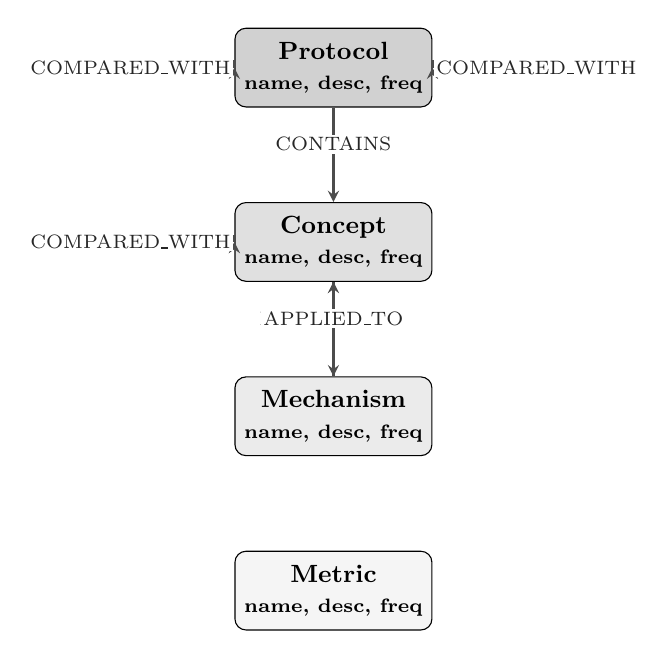
\begin{tikzpicture}[
        node distance=1.2cm and 2cm,
        entity/.style={rectangle, rounded corners=4pt, draw=black, fill=black!#1,
            minimum height=1cm, minimum width=2.2cm, align=center, font=\small\bfseries},
        rel/.style={-{stealth}, thick, draw=black!70},
        rel_label/.style={font=\scriptsize, text=black!85, fill=white, inner sep=1pt}
    ]
    % Entity nodes (灰度差异区分四类实体)
    \node[entity=18] (proto) {Protocol\\{\scriptsize name, desc, freq}};
    \node[entity=12, below=of proto] (conc) {Concept\\{\scriptsize name, desc, freq}};
    \node[entity=8, below=of conc] (mech) {Mechanism\\{\scriptsize name, desc, freq}};
    \node[entity=4, below=of mech] (met) {Metric\\{\scriptsize name, desc, freq}};

    % Relations
    \draw[rel] (proto) -- node[rel_label, above] {CONTAINS} (conc);
    \draw[rel] (conc) -- node[rel_label, above] {DEPENDS\_ON} (mech);
    \draw[rel] (proto.east) to[bend left=30] node[rel_label, right] {COMPARED\_WITH} (proto.east);
    \draw[rel] (mech) -- node[rel_label, above] {APPLIED\_TO} (conc);

    % Self-referencing COMPARED_WITH
    \draw[rel] (proto.west) to[bend left=40] node[rel_label, left] {COMPARED\_WITH} (proto.west);
    \draw[rel] (conc.west) to[bend left=40] node[rel_label, left] {COMPARED\_WITH} (conc.west);
    \end{tikzpicture}
    \caption{Neo4j 图数据库 Schema}\label{fig:3-4}
\end{figure}

每类节点存储 $name$（规范名称，唯一约束）、$description$（实体描述）和 $frequency$（出现频次）。每种关系存储 $frequency$ 和 $evidences$（证据文本列表）。

\textbf{索引与约束。} 在 \texttt{name} 字段上建立唯一性约束，保证同名实体的幂等导入；在 \texttt{frequency} 字段上建立索引以支持按频次的快速排序与高频实体检索。导入采用 Cypher MERGE 语句保证幂等性，重复导入相同三元组不会产生重复节点或边。所有关系附带 \texttt{evidences} 字段，使下游应用在查询时可同步获取支撑证据，保障知识溯源能力。

\subsection{本章小结}

本章阐述了课程知识抽取系统的需求分析和各模块的设计决策。系统设计围绕三条主线：\textit{模块化}——各阶段独立封装、通过文件系统交换中间产物；\textit{可验证性}——证据门控机制要求每条关系附带原文依据，三元组的正确性可自动检验；\textit{混合策略}——别名表与嵌入语义互补完成实体规范化，两阶段抽取平衡召回率与精度。这些设计为第四章的系统总体架构搭建和各模块工程实现奠定了基础。
                   % 第3章 课程知识抽取系统设计（需求分析 → 各模块设计决策与取舍理由）
    \section{系统实现}

本章给出QmrKG系统各模块的具体实现，包括系统总体架构、代码结构、关键参数配置和工程决策。第三章阐述了各模块的设计决策与取舍理由，本章聚焦于“如何实现”——给出六阶段流水线的完整架构、各阶段的配置参数与关键实现细节。

\subsection{系统总体架构}

\subsubsection{六阶段流水线架构}

系统采用六阶段串行流水线，将原始教材逐步转化为结构化知识图谱。六个阶段依次是：文档转图、OCR识别、文本分块、三元组抽取、三元组合并以及图数据库导入，如图\ref{fig:4-1}所示。

\begin{figure}[ht]
    \centering
    \begin{tikzpicture}[
        node distance=0.5cm and 0.15cm,
        stage/.style={
            rectangle, rounded corners=3pt, draw=black, fill=black!10,
            minimum height=0.85cm, minimum width=1.5cm, align=center,
            font=\footnotesize, text=black!90
        },
        data/.style={
            rectangle, rounded corners=2pt, draw=black!60, dashed, fill=black!4,
            minimum height=0.6cm, minimum width=1.3cm, align=center,
            font=\scriptsize, text=black!85
        },
        arr/.style={-{stealth}, thick, draw=black!70},
        darr/.style={-{stealth}, dashed, draw=black!60}
    ]
    % Stages
    \node[stage] (s1) {文档转图\\{\scriptsize PyMuPDF}};
    \node[stage, right=of s1] (s2) {OCR识别\\{\scriptsize VLM}};
    \node[stage, right=of s2] (s3) {文本分块\\{\scriptsize tiktoken}};
    \node[stage, right=of s3] (s4) {三元组抽取\\{\scriptsize LLM}};
    \node[stage, right=of s4] (s5) {三元组合并\\{\scriptsize 别名+嵌入}};
    \node[stage, right=of s5] (s6) {图数据库\\{\scriptsize Neo4j}};

    % Data nodes
    \node[data, below=0.5cm of s1] (d1) {PNG};
    \node[data, below=0.5cm of s2] (d2) {Markdown};
    \node[data, below=0.5cm of s3] (d3) {JSON\\{\scriptsize Chunks}};
    \node[data, below=0.5cm of s4] (d4) {Raw\\{\scriptsize Triples}};
    \node[data, below=0.5cm of s5] (d5) {Merged\\{\scriptsize Triples}};

    % Input
    \node[left=0.5cm of s1, font=\footnotesize, text=black!70] (input) {PDF/PPT};

    % Arrows: input → stages
    \draw[arr] (input) -- (s1);
    \draw[arr] (s1) -- (s2);
    \draw[arr] (s2) -- (s3);
    \draw[arr] (s3) -- (s4);
    \draw[arr] (s4) -- (s5);
    \draw[arr] (s5) -- (s6);

    % Arrows: stages → data
    \draw[darr] (s1) -- (d1);
    \draw[darr] (s2) -- (d2);
    \draw[darr] (s3) -- (d3);
    \draw[darr] (s4) -- (d4);
    \draw[darr] (s5) -- (d5);

    % Data labels
    \node[below=0.15cm of d1, font=\tiny, text=black!60] {data/png/};
    \node[below=0.15cm of d2, font=\tiny, text=black!60] {data/markdown/};
    \node[below=0.15cm of d3, font=\tiny, text=black!60] {data/chunks/};
    \node[below=0.15cm of d4, font=\tiny, text=black!60] {data/triples/raw/};
    \node[below=0.15cm of d5, font=\tiny, text=black!60] {data/triples/merged/};
    \end{tikzpicture}
    \caption{六阶段流水线总体架构}\label{fig:4-1}
\end{figure}

选择六阶段串行架构，主要出于三点考虑：

（1）\textbf{关注点分离}。每个阶段拥有明确的输入契约和输出契约，职责单一。文档转图阶段只负责将PDF/PPT渲染为PNG图像，不关心后续OCR如何处理；OCR阶段只负责图像到文本的转换，不关心文本如何分块。各阶段的独立性使其可以分别设计、测试与演进。

（2）\textbf{模块化与可替换性}。每个阶段对应一个独立的CLI命令（\texttt{pdftopng}、\texttt{pngtotext}、\texttt{mdchunk} 等），阶段之间通过文件系统中的中间产物（PNG、Markdown、JSON）传递数据。保持输入输出格式不变，任何阶段都可以替换实现。例如OCR阶段可从VLM切换为传统OCR引擎，无需改动上下游代码。

（3）\textbf{独立扩展与容错}。中间产物持久化存储在 \texttt{data/} 目录下，流水线天然具备断点续跑能力。若某阶段因API限流或网络故障中断，重新运行该阶段即可从中断点继续，无需从头开始。此外，不同阶段对计算资源的需求差异悬殊——OCR阶段依赖GPU加速的多模态推理，分块阶段仅需CPU计算——独立阶段使资源可按需分配。

\subsubsection{LLM工厂模式}

系统内多个阶段需要调用大语言模型，涉及OCR、实体抽取、关系审核与实体嵌入等任务，各阶段对模型能力、速率限制和提示词策略的要求不同。为此，系统设计了LLM工厂模式（TaskLLMFactory），采用\textbf{任务作用域的配置隔离}。

每个任务（\texttt{ocr}、\texttt{extract}、\texttt{entity\_embed} 等）通过 \texttt{llm\_profile} 字段引用一个预定义的模型配置档案（Profile），档案内包含模型名称、API端点、模态（text/multimodal/embedding）、请求超时、重试策略及速率限制参数。切换模型时只需修改配置文件中的Profile引用，无需改动任何代码。

速率限制采用滑动窗口算法（RollingRateLimiter），维护60秒时间窗口内的请求计数，达到RPM上限后阻塞等待。并发控制通过信号量（Semaphore）实现，确保同时运行的LLM请求数不超过 \texttt{max\_concurrency}。不同任务的速率限制参数可独立配置：OCR任务使用 \texttt{qwen3-vl-8b} 模型，设为RPM 100、并发10；抽取任务使用 \texttt{deepseek\_v4\_flash} 模型，设为RPM 3000、并发3000，以匹配不同模型的配额和吞吐能力。

\subsubsection{流水线配置管理与基础设施}

系统通过统一的 \texttt{config.yaml} 配置文件管理各阶段的模型选型、提示词模板、速率限制和输出路径。配置文件遵循分层结构：\texttt{llm.profiles} 段定义所有可用的模型档案（名称、端点、模态、并发参数），各任务段（\texttt{ocr}、\texttt{extract}、\texttt{entity\_embed}）通过 \texttt{llm\_profile} 键引用档案，并在 \texttt{prompts} 段维护任务特定的提示词。目录路径集中于 \texttt{run} 段，各CLI命令在未显式传参时自动读取配置文件的默认值。

每阶段的CLI命令（\texttt{pdftopng}、\texttt{pngtotext}、\texttt{mdchunk} 等）通过argparse构建参数解析，命令行显式传参会覆盖配置文件默认值。各命令以标准的 \texttt{main()} 函数作为入口，统一模式为：加载配置 $\to$ 解析参数 $\to$ 初始化组件 $\to$ 执行处理 $\to$ 输出结果。所有CLI命令通过项目根目录的 \texttt{pyproject.toml} 注册为 \texttt{[project.scripts]} 入口，用户可通过 \texttt{uv run <command>} 执行。

日志记录采用Python标准库的logging模块，按阶段分别配置INFO和DEBUG两个级别。INFO日志记录各阶段的处理进度、文档数量、已用时间和API调用统计；DEBUG日志记录每个LLM请求的完整payload和响应内容，用于调试提示词和定位异常。日志同时输出到控制台和按日期轮转的日志文件（\texttt{logs/} 目录），保留最近30天的历史记录。出现API调用失败（429或5xx）时，除了重试机制外，还会在日志中记录失败详情（请求ID、错误码、重试次数），便于追踪API稳定性问题。

管道中各阶段均采用ThreadPoolExecutor进行并发处理，由配置文件的 \texttt{max\_concurrency} 字段控制最大并发数。不同阶段的并发数根据下游API的配额独立设置，避免彼此竞争。OCR阶段（并发10）受限于多模态模型的推理吞吐，抽取阶段（并发3000）利用文本模型的高吞吐优势。各线程间通过文件系统中间产物通信，不共享内存状态，避免了锁竞争和数据一致性问题。

\subsection{文档渲染与OCR实现}

\subsubsection{PDF渲染模块}

渲染模块将PDF和PowerPoint文件转为PNG图像，作为VLM OCR的标准化视觉输入。PDF页面通过PyMuPDF（\texttt{fitz} 库）渲染：\texttt{fitz.Matrix(zoom, zoom)} 构造缩放矩阵，\texttt{page.get\_pixmap(matrix)} 获取像素图并保存为PNG，DPI默认为200（$zoom = dpi / 72 \approx 2.78$）。该参数在文字清晰度与文件体积之间取得平衡：DPI过低影响OCR识别质量，DPI过高则导致文件体积过大、处理耗时增加。

对于PPT/PPTX文件，使用LibreOffice无头模式（headless）先转换为临时PDF，再经PDF渲染器统一处理。LibreOffice对Microsoft Office格式的兼容性优于其他开源方案，转换后的PDF保留原始幻灯片的版式和字体信息，确保后续OCR阶段的输入质量。所有PNG按书籍分目录存放于 \texttt{data/png/}，目录结构由文档源文件名自动生成。

\subsubsection{VLM OCR实现}

OCR模块基于Qwen3-VL-8B多模态视觉语言模型，通过PPIO API的OpenAI兼容接口调用。每张PNG图像经Base64编码后，与OCR提示词一同以multipart格式发送。提示词以中文撰写，要求输出有效Markdown、保持原语言不翻译、保留阅读顺序和换行、识别标题层级（\texttt{\#} 一级至 \texttt{\#\#\#} 三级），并对中文教材中常见的章节结构词（“第X章”“第X节”）进行标题化处理。

并发OCR使用ThreadPoolExecutor，并发数由 \texttt{config.yaml} 中的 \texttt{max\_concurrency} 控制（默认10）。每页OCR结果写入独立Markdown文件，文件头部的YAML元数据记录模型名称、Token用量和耗时信息。所有单页Markdown文件由 \texttt{kgmdcombine} 阶段按页码顺序合并为完整的教材级Markdown文档，确保跨页内容的连贯性。

\subsection{文本分块实现}

文本分块模块连接OCR输出与LLM知识抽取入口。系统使用tiktoken库（\texttt{cl100k\_base} 编码）做精确Token计数，同时配备离线安全的字符级近似回退方案。分块算法采用递归标题感知策略（见第三章算法 \ref{al:3-1}），Token上限 $T_{max} = 4000$，优先在标题边界切分，无标题可分时退至段落级累积切分。

实现层面，Markdown解析使用栈式结构处理 \texttt{\#} 标记构建标题树，递归函数 \texttt{chunk\_recursive()} 处理三种情况：子树在预算内则整体输出；超出预算且有子标题则递归下降至子标题层；无子标题则在段落级别按预算累积切分。清洗步骤先去除YAML前置元数据、页码标记和页眉页脚等OCR伪影，再送入分块逻辑。每个输出块记录所属标题层级（\texttt{titles} 字段）、Token数量及源文件信息，供下游抽取阶段做上下文定位。

\subsection{命名实体识别实现}

\subsubsection{LLM工厂与限流机制}

所有LLM调用通过统一的工厂模式（TaskLLMFactory）管理。工厂按任务名称（\texttt{extract}、\texttt{ocr}、\texttt{entity\_embed} 等）从配置文件加载对应的模型参数、API密钥和速率限制策略，返回TaskLLMRunner实例。

TaskLLMRunner集成了请求执行、重试与指数退避。遇到429（速率限制）或5xx（服务端错误）时自动指数退避重试（首次1s，逐次翻倍，上限由 \texttt{max\_retries} 配置，默认5次）。RollingRateLimiter使用滑动窗口算法，统计60秒内请求数，达到RPM上限后阻塞等待，避免触发服务端限流。每次LLM调用记录耗时和Token用量，便于性能监控和成本核算。

\subsubsection{两阶段抽取流程}

知识抽取采用Propose--Review两阶段架构，其设计依据见第三章。实现上，两阶段均为独立的LLM调用：

\textbf{提议阶段：} LLM接收文本块和完整的Schema定义（实体类型表 \ref{tab:3-1}、关系类型表 \ref{tab:3-2}）及对应模式的提示词，输出JSON格式的候选实体列表（含name、type、description字段）和三元组列表（含head、relation、tail、evidence字段）。此阶段侧重召回率。

\textbf{审核阶段：} 通过一次独立的LLM调用，对每个候选三元组逐一验证。审核提示词要求LLM逐项检查以下五条规则：（1）关系类型是否属于预定义的四种之一；（2）evidence字段是否为文本块中的连续原文子串且逐字一致；（3）头实体和尾实体是否均出现在evidence字段中；（4）head与tail是否相同（自环检测）；（5）是否引入了文本块中不存在的新实体。每个三元组的审核结果包含 $decision$（keep / revise / drop）和 $reason\_code$（如SUPPORTED、EVIDENCE\_NOT\_IN\_CHUNK、HEAD\_NOT\_IN\_EVIDENCE、SELF\_LOOP等）。

系统对每个文本块依次执行提议和审核，未通过证据门控的三元组被丢弃或标记为修正。所有中间结果以JSON格式持久化存储，支持调试和结果复现。

\subsubsection{抽取模式与提示词管理}

系统支持Zero-shot和Few-shot两种抽取模式，通过命令行 \texttt{--mode} 参数切换。两种模式的提示词存放在 \texttt{config.yaml} 的 \texttt{extract.prompts} 配置段中，支持热更新——修改配置文件后重新运行即可应用新提示词，无需改动代码。

Zero-shot模式提示词包含三个核心组件：Schema定义（四种实体类型的名称、定义及示例）、抽取规则（仅从给定文本中抽取、不编造实体、使用原文名称）和输出格式约束（严格JSON，包含entities和triples数组）。Few-shot模式在Zero-shot基础上额外加载四个标注示例（每种关系类型一个）和粒度规则的负面示例（不抽取过泛词如“计算机”“网络”“系统”），以抑制过度抽取倾向并提升跨文档的一致性。

抽取过程使用ThreadPoolExecutor并行化，并发度由 \texttt{max\_concurrency} 控制。每个文本块的抽取结果保存为独立JSON文件，Zero-shot和Few-shot模式分目录存放（\texttt{data/triples/raw/zs/} 和 \texttt{data/triples/raw/fs/}），支持结果对比与模式切换。

\subsection{关系抽取实现}

\subsubsection{Propose--Review流程实现}

关系抽取与实体识别共用同一套提示词和两阶段架构，在提议阶段同时输出实体和关系，在审核阶段对三元组进行独立的验证。审核阶段的实现利用了第三章定义的evidence验证规则：系统在原始文本块中搜索evidence子串（通过Python \texttt{str.find()} 实现），找到则保留，未找到则丢弃。这一“字符串匹配门控”的实现简洁高效，不依赖额外的LLM调用或模型推理。

实际运行中发现，审核阶段不仅过滤了虚假关系，还能通过reason\_code提供诊断信息。例如，EVIDENCE\_NOT\_IN\_CHUNK提示evidence字段与原文不匹配，可能是LLM在生成evidence时进行了改写或合并；HEAD\_NOT\_IN\_EVIDENCE提示实体识别与关系抽取的边界不一致。这些诊断信息为持续优化提示词提供了反馈。

\subsubsection{关系约束与置信度}

审核阶段输出的三元组还需通过类型约束检查：头尾实体的类型组合必须符合关系Schema表（参见第三章表 \ref{tab:3-2}）中定义的类型约束。例如，compared\_with限定头尾实体为同类型（protocol ↔ protocol或concept ↔ concept），applied\_to限定头实体为mechanism。不符合约束的三元组被标记为REVISED，并将关系类型调整为可能的替代选项。通过检查的三元组记录 $confidence$ 分数字段（基于evidence长度与文本块长度的比率及审核阶段的reason\_code计算），为后续知识融合提供质量依据。

\subsection{知识融合实现}

\subsubsection{实体别名规范化}

从多个文本块中抽取的实体存在名称变体（“传输控制协议”“TCP协议”“TCP”等）。系统通过别名映射表（ALIAS\_MAP）和正则后缀剥离实现Level 1规范化。映射表包含50余条中英文缩写与全称对应关系（如 \texttt{"传输控制协议" → "TCP"}、\texttt{"往返时延" → "RTT"}），同时通过正则 \texttt{(协议|算法|机制|方法|技术|方式)\$} 剥离实体名称末尾的类型后缀。规范化后将名称与类型组成复合键进行合并，保留最高频名称和首个非空描述，累加频次。

\subsubsection{基于嵌入的语义规范化}

别名表只能覆盖词典阶段已知的同义关系，难以处理抽取过程中产生的长尾变体，例如术语翻译差异（“快速重传”与“快速重发”）、修饰成分差异（“基于丢包的拥塞控制”与“丢包驱动的拥塞控制算法”）以及OCR残留引入的字符级噪声。系统因此引入基于嵌入向量的语义规范化（Level 2）作为兜底机制。EmbeddingCanonicalizer通过LLM工厂的 \texttt{EmbeddingTaskProcessor} 调用嵌入模型（向量维度1024）将每个实体编码为语义向量，1024维在表达能力和FAISS索引内存占用之间取得平衡。

编码文本采用结构化模板“实体类型：\{type\}；实体名：\{name\}；定义：\{description\}”，把类型字段和描述字段同时纳入上下文。纯名称编码会忽略学科语境——例如“窗口”在protocol桶中应贴近“滑动窗口”，在metric桶中应贴近“拥塞窗口大小”，仅以名称为输入难以区分；引入类型与描述后，向量同时承载类别与语义信息，可有效抑制跨类型误合并。流程如算法 \ref{al:4-1} 所示。

\begin{algorithm}[H]
    \caption{基于FAISS的嵌入实体规范化}\label{al:4-1}
    \begin{algorithmic}[1]
        \Require 实体列表 $E$，相似度阈值 $\theta$，编码模板 $T$
        \Ensure 规范化实体集合 $E'$
        \State 按实体类型分桶（可选）：$E_{type} \gets \{e \in E \mid e.type = type\}$
        \For{each桶 $B$}
            \State 对每个实体 $e \in B$，构建编码文本：
            \Statex \hspace{2em} $T(e) \gets$ ``实体类型：\{$e.type$\}；
            \Statex \hspace{4em} 实体名：\{$e.name$\}；
            \Statex \hspace{4em} 定义：\{$e.description$\}''
            \State 调用Embedding API获取向量 $v_e$
            \State 构建FAISS IndexFlatIP索引（余弦相似度，内积归一化）
            \State 对每个实体查询 $top\_k$ 最相似实体
            \State 使用并查集（UnionFind）合并相似度 $\geq \theta$ 的实体对
            \State 选择规范代表名：频率最高 $\to$ 名称最短 $\to$ 字典序最小
        \EndFor
        \State \Return $E'$
    \end{algorithmic}
\end{algorithm}

选择FAISS IndexFlatIP作为向量索引的原因：（1）FAISS提供高效的近似最近邻搜索，适用于数万级实体集合；（2）IndexFlatIP内积搜索配合向量归一化即可实现余弦相似度计算，无需额外索引类型；（3）FAISS的批量查询接口与ThreadPoolExecutor并发架构兼容，避免了向量搜索成为流水线瓶颈。

相似度阈值 $\theta$ 设为0.85。阈值过低会将语义不同的实体错误合并（如“拥塞控制”与“流量控制”），阈值过高则无法合并真正的同义变体（如“TCP协议”与“TCP”）。实验表明0.85在两者之间取得了平衡。

嵌入缓存机制（\_EmbeddingBinaryCache）将已计算的嵌入向量序列化为NumPy二进制文件（.npy）和JSON元数据文件。缓存以实体名称和类型的哈希作为键，避免对相同实体重复调用Embedding API。大规模规范化场景下（数千实体），缓存可降低70\% 以上的API调用量。

\subsubsection{三元组合并与去重}

实体规范化完成后，以规范化后的（$head$, $relation$, $tail$）三元组为键分组，累加频次并收集全部 $evidences$ 列表。合并后过滤自环三元组（$head = tail$）及头尾实体不在有效实体集合中的三元组。合并结果写入 \texttt{merged\_triples.json}，Zero-shot和Few-shot结果分目录存放，结构为 \texttt{\{"entities": [...], "triples": [...]\}}。

\subsection{Neo4j图数据库导入实现}

\subsubsection{Cypher批量导入}

KGNeo4jLoader基于neo4j Python驱动（Bolt协议）执行导入。连接参数（\texttt{NEO4J\_URI}、\texttt{NEO4J\_USER}、\texttt{NEO4J\_PASSWORD}）从环境变量读取，通过 \texttt{GraphDatabase.driver()} 建立连接。导入流程分两步执行：第一步，按实体类型创建不同标签的节点（Protocol、Concept、Mechanism、Metric），以 $name$ 字段作为唯一约束；第二步，按关系类型创建有向边（CONTAINS、DEPENDS\_ON、COMPARED\_WITH、APPLIED\_TO），以头尾节点对和关系类型匹配。

使用Cypher MERGE语句保证幂等性——重复导入相同数据不会产生重复节点或边。每条边额外存储 $frequency$ 和JSON格式的 $evidences$ 数组。批量写入采用 \texttt{execute\_query} 配合参数化查询，针对数千条三元组的导入可在秒级完成。导入前可通过 \texttt{--clear} 参数清空已有数据库，便于重复实验。

\subsubsection{索引、约束与查询接口}

为支持下游应用按实体类型与频次的高效检索，导入阶段同时为四类节点标签的 \texttt{name} 字段建立唯一性约束，为 \texttt{frequency} 字段建立B+ 树索引。约束保证幂等导入下不产生重名实体，索引则将“按频次取前 $N$ 个高频节点并查询其诱导子图”等典型查询的耗时控制在毫秒级。完成导入后，用户可通过Neo4j Browser或Bolt协议驱动直接执行Cypher查询，按实体类型、关系类型或频次条件检索知识子图，每条返回的关系附带 \texttt{evidences} 字段以保留原文证据，便于后续应用集成。

\subsection{本章小结}

本章给出了QmrKG各模块的完整实现细节。系统总体架构采用六阶段串行流水线，各阶段以CLI命令暴露并通过文件系统中间产物解耦；LLM工厂模式通过任务作用域配置隔离统一管理OCR、抽取和嵌入三类LLM调用，配合滑动窗口速率限制和指数退避重试保障稳定性。文档渲染使用PyMuPDF（DPI 200）和LibreOffice无头模式；OCR基于Qwen3-VL-8B并通过ThreadPoolExecutor并发处理；文本分块采用递归标题感知策略，Token上限4000。知识抽取实现两阶段Propose--Review架构，审核阶段执行五条证据验证规则；知识融合结合别名映射表（50余条）和FAISS嵌入语义规范化（阈值0.85），嵌入结果通过二进制缓存复用。Neo4j导入使用Cypher MERGE幂等操作，配合 \texttt{name} 唯一约束与 \texttt{frequency} 索引支持下游应用的高效查询。
           % 第4章 系统实现（总体架构 → 文档渲染与OCR → 文本分块 → NER → RE → 知识融合 → 图存储与可视化）
    \section{实验与结果分析}

大语言模型评测需要结合任务场景、评价指标和输出可靠性设计评价口径\cite{luowen2024_llm_eval}。本章围绕基于大模型的课程知识实体识别与关系抽取系统，报告实验设计与运行结果。先介绍实验环境与配置参数，随后从课程语料构建、实体抽取评估、关系抽取评估、零样本与少样本抽取对比评估、知识图谱质量分析以及典型案例分析等角度，对系统运行结果进行评估与讨论。

\subsection{实验环境与配置}

本实验在统一的软硬件环境下运行，实验配置如表~\ref{tab:5-1}所示。硬件选用计算能力较强的服务器，软件环境基于Python 3.13，使用uv作为包管理器。系统核心依赖大语言模型API完成OCR识别、知识抽取与向量化表示三类任务。

\begin{table}[ht]
    \centering
    \caption{实验软硬件环境配置}
    \label{tab:5-1}
    \begin{tabular}{llp{8cm}}
    \toprule
    \textbf{配置类别} & \textbf{配置项} & \textbf{参数值} \\
    \midrule
    \multirow{3}{*}{硬件配置}
    & CPU & x86\_64架构多核处理器 \\
    & 内存 & 32GB DDR4 \\
    & 存储 & SSD固态硬盘 \\
    \midrule
    \multirow{3}{*}{软件环境}
    & 操作系统 & Linux (Ubuntu 24.04 LTS) \\
    & Python版本 & 3.13 \\
    & 包管理器 & uv \\
    \midrule
    \multirow{3}{*}{LLM配置}
    & OCR模型 & qwen3-vl-8b \\
    & 抽取模型 & deepseek-v4-flash \\
    & 嵌入模型 & qwen3-embedding-8b（向量维度1024） \\
    \bottomrule
    \end{tabular}
\end{table}

表~\ref{tab:5-2}列出了流水线核心参数配置。PDF渲染选用200 DPI分辨率以兼顾OCR识别质量；文本分块最大token数设为4000，平衡上下文完整性与处理效率；知识抽取采用few-shot模式提高准确性；同时启用严格证据验证机制，要求所有抽取得到的三元组均可溯源至原文。

\begin{table}[ht]
    \centering
    \caption{流水线核心参数配置}
    \label{tab:5-2}
    \begin{tabular}{llp{6cm}}
    \toprule
    \textbf{处理阶段} & \textbf{参数项} & \textbf{参数值} \\
    \midrule
    PDF转PNG & DPI分辨率 & 200 \\
    \midrule
    文本分块 & 最大token数 & 4000 \\
    & 分块策略 & 语义边界感知 \\
    \midrule
    知识抽取 & 抽取模式 & few-shot (fs) \\
    & 证据审查 & enabled \\
    & 严格证据 & enabled \\
    \midrule
    并发处理 & OCR并发数 & 10 \\
    & 抽取并发数 & 4 \\
    & 执行器类型 & ThreadPoolExecutor \\
    \bottomrule
    \end{tabular}
\end{table}

本实验使用ThreadPoolExecutor对OCR识别与知识抽取两个阶段进行并行加速。OCR阶段并发数设为10，知识抽取阶段并发数设为4，该配置在API速率限制与处理效率之间取得了平衡。

\subsection{课程语料构建结果}

本实验构建了覆盖计算机网络课程全内容的多元化语料库。根据\texttt{data/pdf}目录下的实际源文件统计，语料来源包括课程课件与讲义、RFC协议标准、实验与编程材料、作业与考核材料以及教材参考书，如表~\ref{tab:5-3}所示。

\begin{table}[H]
    \centering
    \caption{课程语料来源构成}
    \label{tab:5-3}
    \begin{tabular}{lp{8cm}r}
    \toprule
    \textbf{来源类型} & \textbf{具体内容} & \textbf{数量} \\
    \midrule
    课程课件与讲义 & 课程介绍、章节讲义、UnderHIT课件、Kurose配套章节课件等 & 115份 \\
    RFC/协议标准文档 & TCP/IP、HTTP、TLS、DNS、IPv6等相关RFC文档 & 72份 \\
    实验与编程材料 & Wireshark实验、Socket编程、实验指导书与FAQ等 & 44份 \\
    作业与考核材料 & Assignment、课后作业、历年试卷、模拟题、答案与解析等 & 33份 \\
    教材与参考书 & 谢希仁《计算机网络》、Kurose \& Ross《自顶向下方法》、《TCP/IP详解》系列及复习资料等 & 19份 \\
    \midrule
    \textbf{总计} & 205份PDF、69份PPT/PPTX、9份Markdown源文件 & \textbf{283份} \\
    \bottomrule
    \end{tabular}
\end{table}

语料库构建结果统计如表~\ref{tab:5-4}所示。在283份源文件中，205份PDF文档进入PDF渲染与OCR流程，并生成274个PNG输出目录（每一个目录对应一个PDF页码集合）。系统最终产生了16,438个语义文本块，总token数达10,398,922，平均每块632.6个token。

\begin{table}[ht]
    \centering
    \caption{语料库构建统计结果}
    \label{tab:5-4}
    \begin{tabular}{lr}
    \toprule
    \textbf{统计指标} & \textbf{数值} \\
    \midrule
    输入PDF文档数 & 205份 \\
    PNG输出目录数 & 274个 \\
    生成文本块数 & 16,438个 \\
    总token数 & 10,398,922 \\
    平均每块token数 & 632.6 \\
    \bottomrule
    \end{tabular}
\end{table}

按进入OCR流程的205份PDF文档计算，平均每份PDF产生约80个文本块。PPT/PPTX与Markdown源文件主要用于补充课程课件、实验说明和章节文本，教材与讲义的内容量较大。语料覆盖中英文双语材料，既有中文教材的系统阐述，也有英文RFC文档的原始技术规范，表明pipeline对多样化课程资源具备处理能力。

\subsection{实体抽取评估}

本实验从16,438个文本块中抽取了实体23,600个，实体类型分布如表~\ref{tab:5-5}所示。系统采用四分类实体模式：concept（概念）、mechanism（机制）、protocol（协议）、metric（性能指标）。

\begin{table}[ht]
    \centering
    \caption{实体类型分布统计}
    \label{tab:5-5}
    \begin{tabular}{lrrl}
    \toprule
    \textbf{实体类型} & \textbf{数量} & \textbf{占比} & \textbf{典型示例} \\
    \midrule
    概念(concept) & 16,719 & 70.8\% & 拥塞控制、流量控制、路由选择 \\
    机制(mechanism) & 3,063 & 13.0\% & 滑动窗口、CRC校验、三次握手 \\
    协议(protocol) & 2,189 & 9.3\% & TCP、UDP、HTTP、IP \\
    性能指标(metric) & 1,629 & 6.9\% & RTT、吞吐量、丢包率、带宽 \\
    \midrule
    \textbf{总计} & \textbf{23,600} & \textbf{100\%} & — \\
    \bottomrule
    \end{tabular}
\end{table}

表~\ref{tab:5-5}显示，概念类型实体占比最高(70.8\%)，这与课程材料以阐述抽象网络概念与原理为主的特性一致。机制类型实体占13.0\%，课程对实现技术给予了相当篇幅。协议类型实体仅占9.3\%，但协议在网络通信中处于基础地位，数量占比不反映其重要程度。性能指标类型实体占6.9\%，覆盖了网络性能评估的主要维度。

高频实体分布如表~\ref{tab:5-6}所示。TCP以2,657次的出现频率排在第一，UDP(1,411次)、IP(1,020次)位列其后，三者是网络协议栈的基础协议。

\begin{table}[ht]
    \centering
    \caption{高频实体统计（Top 10）}
    \label{tab:5-6}
    \begin{tabular}{lrclr}
    \toprule
    \textbf{排名} & \textbf{实体} & \textbf{频次} & \textbf{类型} & \textbf{占比*} \\
    \midrule
    1 & TCP & 2,657 & protocol & 11.3\% \\
    2 & UDP & 1,411 & protocol & 6.0\% \\
    3 & IP & 1,020 & protocol & 4.3\% \\
    4 & HTTP & 932 & protocol & 3.9\% \\
    5 & DNS & 723 & protocol & 3.1\% \\
    6 & RTT & 551 & metric & 2.3\% \\
    7 & IPv6 & 521 & protocol & 2.2\% \\
    8 & ICMP & 492 & protocol & 2.1\% \\
    9 & IPv4 & 469 & protocol & 2.0\% \\
    10 & OSPF & 451 & protocol & 1.9\% \\
    \bottomrule
    \multicolumn{5}{l}{\small *占总实体数的百分比}
    \end{tabular}
\end{table}

实体出现频次的范围为1至2,657，平均频次3.9次，呈典型的长尾分布。前10个高频实体累计占比约38\%，超过半数的实体(约12,000个)仅出现1～2次。该分布遵循幂律规律：高频术语在网络课程文献中被反复讨论，低频术语仅在特定上下文中出现。

TCP、UDP、IP等高频协议实体的频次远超均值，与它们在网络课程中的教学重心一致。系统识别了四类实体，为后续关系抽取与知识图谱构建提供了输入。

\subsection{关系抽取评估}

从23,600个实体中，本实验抽取了关系三元组44,526个。关系类型采用四分类体系：contains（包含）、applied\_to（应用于）、depends\_on（依赖于）、compared\_with（比较于），分布统计如表~\ref{tab:5-7}所示。

\begin{table}[ht]
    \centering
    \caption{关系类型分布统计}
    \label{tab:5-7}
    \begin{tabular}{lrr}
    \toprule
    \textbf{关系类型} & \textbf{数量} & \textbf{占比} \\
    \midrule
    包含(contains) & 15,251 & 34.3\% \\
    应用于(applied\_to) & 14,291 & 32.1\% \\
    依赖于(depends\_on) & 9,601 & 21.6\% \\
    比较于(compared\_with) & 5,383 & 12.1\% \\
    \midrule
    \textbf{总计} & \textbf{44,526} & \textbf{100\%} \\
    \bottomrule
    \end{tabular}
\end{table}

contains与applied\_to两类合计占66.4\%，反映了教育内容在知识结构上的两个特征：既强调概念的层级包含关系(如"TCP包含拥塞控制")，也关注机制的具体应用场景(如"滑动窗口应用于TCP")。depends\_on关系占21.6\%，源自网络协议栈的层次依赖特性(如"HTTP依赖于TCP")。

compared\_with关系占比最低(12.1\%)。比较分析属于高阶认知任务，在基础教材中出现频率较低，但这类关系表达了概念间的对比与区别，对完整描述课程知识结构是必要的。

高频三元组统计如表~\ref{tab:5-8}所示。

\begin{table}[ht]
    \centering
    \caption{高频关系三元组统计（Top 5）}
    \label{tab:5-8}
    \begin{tabular}{lcr}
    \toprule
    \textbf{关系三元组} & \textbf{频次} & \textbf{关系类型} \\
    \midrule
    TCP \textit{compared\_with} UDP & 421 & 比较 \\
    TCP \textit{contains} 拥塞控制 & 133 & 包含 \\
    IPv6 \textit{compared\_with} IPv4 & 130 & 比较 \\
    HTTP \textit{depends\_on} TCP & 122 & 依赖 \\
    TCP \textit{depends\_on} IP & 75 & 依赖 \\
    \bottomrule
    \end{tabular}
\end{table}

TCP与UDP之间的比较关系出现最为频繁：双向比较(TCP↔UDP)累计超过600次，说明传输层协议对比是课程反复涉及的话题。IPv6与IPv4的比较关系出现130次，与网络层协议演进的教学内容直接相关。

本实验启用了严格证据验证机制(strict\_evidence enabled)，所有三元组均附带可追溯的原文证据。该机制过滤了无依据的虚假关系，确保每条三元组均可回溯到源文本。

\subsection{零样本与少样本抽取对比评估}

为了让zero-shot（zs）与few-shot（fs）的抽取结果可以进行公平比较，本实验没有把任一模式的预测结果直接作为金标来源，而是以\texttt{data/chunks}中的原始文本块为回溯对象，构建并复核独立评估集。当前用于评估的金标文件为\texttt{data/eval/gold\_triples.json}，它与\texttt{data/eval/gold\_triples.500\_reviewed.json}内容一致，包含500条关系三元组和594个实体，覆盖88个源文件以及186个源文本块。核查过程中逐条检查了\texttt{source\_file}、\texttt{chunk\_index}与\texttt{evidence}字段：所有源文件均存在，所有chunk索引均有效，500条证据文本均为对应源文本块中的连续原文子串。其中有17条证据最初只是空白折叠后的文本，已替换为带原始换行的精确片段。

评估采用系统中的\texttt{kgeval}严格匹配口径。实体匹配要求实体名与类型完全一致，三元组匹配要求\texttt{head}、\texttt{head\_type}、\texttt{relation}、\texttt{tail}和\texttt{tail\_type}五个字段完全一致，不进行别名归一化、大小写折叠、后缀剥离或向量语义匹配。为了避免用全量图谱去对比500条抽样金标时把大量未标注但可能正确的关系误计为假阳性，实验先把四种raw抽取输出过滤到金标覆盖的186个源文本块，再在关闭embedding合并的条件下执行\texttt{kgmerge}，最后用同一份金标计算指标。该口径把比较范围限制在相同文本证据范围内，适合观察zs/fs提示方式和复核开关对严格命中的影响。

\begin{table}[ht]
    \centering
    \caption{零样本与少样本抽取在500条金标上的严格匹配结果}
    \label{tab:5-zsfs}
    \resizebox{\textwidth}{!}{
    \begin{tabular}{lrrrrrrrrr}
    \toprule
    \textbf{模式} & \textbf{Raw文件} & \textbf{Raw三元组} & \textbf{合并三元组} & \textbf{实体P} & \textbf{实体R} & \textbf{实体F1} & \textbf{三元组P} & \textbf{三元组R} & \textbf{三元组F1} \\
    \midrule
    \texttt{zs-nocheck} & 184 & 418 & 337 & 26.95\% & 51.68\% & 35.43\% & 18.99\% & 12.80\% & 15.29\% \\
    \texttt{zs-recheck} & 182 & 397 & 314 & 27.45\% & 51.35\% & 35.78\% & 17.83\% & 11.20\% & 13.76\% \\
    \texttt{fs-nocheck} & 171 & 325 & 290 & 24.36\% & 44.95\% & 31.60\% & 16.21\% & 9.40\% & 11.90\% \\
    \texttt{fs-recheck} & 176 & 392 & 304 & 26.04\% & 45.29\% & 33.07\% & 15.79\% & 9.60\% & 11.94\% \\
    \bottomrule
    \end{tabular}
    }
\end{table}

表~\ref{tab:5-zsfs}显示，在严格三元组匹配口径下，\texttt{zs-nocheck}的三元组F1最高（15.29\%），三元组精确率和召回率也高于另外三种设置；\texttt{zs-recheck}的实体F1最高（35.78\%）。在few-shot设置内部，启用复核后实体F1从31.60\%升至33.07\%，三元组召回率从9.40\%升至9.60\%，但三元组精确率从16.21\%降至15.79\%，说明复核在保留更多候选关系的同时，也引入了更多未被严格金标命中的三元组。

本实验中的金标是经人工复核的正例参考集，并非对186个源文本块中所有可能正确关系的穷尽标注。因此，表中的精确率应理解为保守的严格重合精确率，不等于完整语义精确率；召回率反映系统对500条已接受金标三元组的严格覆盖能力。在当前提示词和严格匹配条件下，zero-shot输出比few-shot更接近金标标注风格，后续优化应聚焦few-shot示例与金标标注规范的一致性，而非单纯增加示例数量。

为了直接衡量两种提示策略在抽取阶段的原始能力，本实验设计了\textbf{原始抽取层面}的逐块评估方案，使用专用的\texttt{kgevalraw}评测工具，在未经过合并的raw三元组上直接与金标进行逐块对比。评估维度涵盖实体层面F1（匹配键：name + type）、三元组层面F1（head、head\_type、relation、tail、tail\_type五字段严格匹配）和关系层面F1（仅匹配head\_type、relation、tail\_type），以及head\_type、tail\_type、relation三个属性的分类准确率。

表~\ref{tab:5-raw-zsfs}展示了zero-shot与few-shot在三个scope层面的精确率、召回率与F1值对比。

\begin{table}[ht]
    \centering
    \caption{原始抽取层面zero-shot与few-shot的scope级指标对比}
    \label{tab:5-raw-zsfs}
    \begin{tabular}{llrrrr}
    \toprule
    \textbf{Scope} & \textbf{Metric} & \textbf{ZS} & \textbf{FS} & \textbf{$\Delta$ (FS$-$ZS)} \\
    \midrule
    \multirow{3}{*}{Entity} & Precision & 40.00\% & 36.90\% & $-$3.10个百分点 \\
    & Recall    & 28.62\% & 27.27\% & $-$1.35个百分点 \\
    & \textbf{F1} & \textbf{33.37\%} & 31.36\% & $-$2.00个百分点 \\
    \midrule
    \multirow{3}{*}{Triple} & Precision & 16.44\% & 13.35\% & $-$3.09个百分点 \\
    & Recall    & 12.00\% & 9.80\% & $-$2.20个百分点 \\
    & \textbf{F1} & \textbf{13.87\%} & 11.30\% & $-$2.57个百分点 \\
    \midrule
    \multirow{3}{*}{Relation} & Precision & 55.00\% & 53.85\% & $-$1.15个百分点 \\
    & Recall    & 80.49\% & 68.29\% & $-$12.20个百分点 \\
    & \textbf{F1} & \textbf{65.35\%} & 60.22\% & $-$5.13个百分点 \\
    \bottomrule
    \end{tabular}
\end{table}

属性分类方面，ZS的head\_type准确率（86.67\%）与FS（84.93\%）接近，但FS在tail\_type上显著领先（89.04\% vs 75.24\%，+13.80个百分点），relation准确率两者相当（85.71\% vs 86.30\%）。

覆盖方面，ZS在186个金标块中找到182个对应raw文件（缺失4个），FS找到176个（缺失10个）。

实验结果显示：（1）Zero-shot在全部三个scope层面的F1指标上均优于few-shot（Entity F1: 33.37\% vs 31.36\%，Triple F1: 13.87\% vs 11.30\%，Relation F1: 65.35\% vs 60.22\%），与合并评估结论一致，说明zero-shot输出更接近金标标注风格。（2）Triple F1与Relation F1差距悬殊（零样本下65.35\% vs 13.87\%），源于实体名称严格匹配：当LLM使用原文完整表述（如"传输控制协议"）而金标使用缩写（"TCP"）时，大量语义正确但字符串不匹配的三元组被计为假阴性。（3）Few-shot仅在tail\_type分类上优于zero-shot（89.04\% vs 75.24\%，+13.80个百分点），但抽取缺失更多（10个vs 4个金标块找不到对应raw文件）。

\subsection{知识图谱质量分析}

在44,526个关系三元组的基础之上，本实验构建了包含23,600个节点、44,526条边的课程知识图谱。图谱的基本统计指标如表~\ref{tab:5-9}所示。

\begin{table}[ht]
    \centering
    \caption{知识图谱基本统计指标}
    \label{tab:5-9}
    \begin{tabular}{lr}
    \toprule
    \textbf{统计指标} & \textbf{数值} \\
    \midrule
    实体节点数 & 23,600 \\
    关系边数 & 44,526 \\
    平均节点度数 & 3.77 \\
    实体平均出现频次 & 3.9次 \\
    高频实体占比(Top 10) & 38\% \\
    \bottomrule
    \end{tabular}
\end{table}

平均节点度数约3.8，与课程知识中高频术语多连接、低频术语少连接的组织规律一致。系统通过词汇级别名表和语义级嵌入向量双层归一化处理实体名称变体，并以TCP等高频协议为枢纽连接多个子概念与关系。

\subsection{案例分析}

本节选取两个典型子图进行分析。TCP协议子图包含对比关系（TCP \textit{compared\_with} UDP，双向616次）、包含关系（TCP \textit{contains} 拥塞控制133次、流量控制89次）和依赖关系（HTTP \textit{depends\_on} TCP 122次、TCP \textit{depends\_on} IP 75次），覆盖协议对比、内部机制和协议栈依赖三个知识维度。协议演进对比子图展示了IPv6 \textit{compared\_with} IPv4（130次）等课程核心对比主题，系统通过统计频次有效识别出教学重点。


\subsection{本章小结}

本章对系统进行了实验评估。系统构建出包含23,600个实体和44,526个关系三元组的课程知识图谱，实体分布以概念类型为主（70.8\%），关系分布以contains和applied\_to为主（66.4\%），平均节点度数3.8。零样本与少样本对比表明，zero-shot在当前提示词与严格匹配条件下整体优于few-shot（合并层面三元组F1: 15.29\% vs 11.94\%，原始层面: 13.87\% vs 11.30\%），few-shot在tail\_type分类上具有局部优势（89.04\% vs 75.24\%）。
              % 第5章 实验与结果分析
    \section{总结与展望}

本研究围绕课程知识的命名实体识别与关系抽取，研究了大语言模型在计算机网络课程知识图谱自动化构建中的应用，完成的工作包括以下几个方面：

（1）在课程语料构建与预处理方面，实现了一套面向计算机网络课程的多源语料自动化预处理流程。语料覆盖教材（谢希仁《计算机网络》第8版\cite{xiexiren2021}、Kurose\&Ross《计算机网络：自顶向下方法》第8版、《TCP/IP详解》等）、课堂讲义（9章课件及10次授课讲稿）、实验指导书、历年试题以及50余份RFC标准文档，共205份PDF文档。预处理阶段使用PyMuPDF渲染PDF页面，LibreOffice无头模式处理PPT/PPTX格式文档，Qwen3-VL-8B多模态视觉语言模型执行OCR文字提取，最终输出结构化Markdown文本。该语料库覆盖多种来源与格式，为后续知识抽取阶段提供了基础。

（2）在命名实体识别方面，本课题为计算机网络领域定义了四类实体：协议名称（protocol，如TCP、HTTP、OSPF）、概念术语（concept，如拥塞控制、子网掩码、分层模型）、机制算法（mechanism，如三次握手、慢启动、CSMA/CD）和性能指标（metric，如吞吐量、RTT、丢包率）。考虑到课程领域缺乏标注数据，研究了零样本（zero-shot）和少样本（few-shot）两种提示策略。零样本模式通过详细的实体类型定义与标注指南引导模型行为；少样本模式在此基础上增加了四条覆盖全部关系类型的标注示例以及负面示例，改进模型对课程术语边界的识别。在启用LLM复核（\texttt{fs-recheck}）的最终配置下抽取并合并得到32,760个实体，频次跨度从1次到2,117次（平均3.32次），高频实体如TCP（2,117次）、UDP（1,069次）、HTTP（701次）、IP（640次）等，分布与计算机网络课程的知识结构大体一致。

（3）在关系抽取方面，本课题定义了四类关系类型：包含关系（contains），表达概念或协议间的结构组成；依赖关系（depends\_on），表示功能实现上的前置条件；对比关系（compared\_with），描述同类实体间的异同；应用关系（applied\_to），说明机制算法在具体协议或场景中的部署方式。抽取架构上，设计了Propose--Review“提议—审核”两阶段流程：第一阶段由大语言模型按Schema生成候选三元组；第二阶段通过独立审核提示词进行质量门控，逐条检查证据是否为输入文本的连续原文子串、头尾实体是否均出现在证据中、关系类型是否合法。该机制要求每条三元组给出可回溯的原文证据，减少了模型生成不实内容的情况。知识融合阶段，通过别名映射表（如“传输控制协议”→“TCP”）以及基于FAISS索引的嵌入语义规范化（结合UnionFind算法）实现跨文档实体消歧。最终知识图谱（\texttt{merged-fs-recheck}）包含32,760个节点和17,627条边，连通子图（13,018个节点）平均度数约2.71。在500条独立金标上采用“严格／软匹配／槽位／类型级”四档匹配口径评估，软匹配三元组F1为15\%~19\%、槽位F1为37\%~42\%、类型级F1可达74\%~82\%。从严格档到类型级档的阶梯说明系统失分主要源于实体表面形式差异，而非关系类型识别错误。

（4）在知识抽取管线方面，本课题构建了六阶段端到端自动化流程：文档渲染（PDF$\rightarrow$PNG）$\rightarrow$OCR文字提取（PNG$\rightarrow$Markdown）$\rightarrow$文本分块（Markdown$\rightarrow$JSON Chunks）$\rightarrow$三元组抽取（Chunks$\rightarrow$Raw Triples）$\rightarrow$知识融合（Raw Triples$\rightarrow$Merged Triples）$\rightarrow$图数据库导入（Merged Triples$\rightarrow$Neo4j）。流水线采用工厂模式统一管理LLM调用，通过滑动窗口速率限制和指数退避重试保障API调用稳定性。各阶段经中间文件解耦，支持断点续跑与独立调试。图存储层面，融合后的三元组通过Cypher MERGE语句幂等导入Neo4j，配合 \texttt{name} 唯一约束与 \texttt{frequency} 索引为下游应用提供基于实体类型、关系类型与频次的高效检索能力。系统验证了大语言模型在课程知识建模中的可行性。

               % 第6章 总结与展望
    
    \include{body/references}               % 参考文献
    \acknowledgement

时光荏苒，转眼就到本科毕业的时候了。这篇论文的完成，离不开许多人的帮助，在这里一一感谢。

首先要感谢我的指导老师。从选题到方案设计，从实验调试到论文撰写，老师在每个阶段都给了我很多具体的指导。老师的严谨和对问题的判断力，我一直很佩服，也跟着学了不少。遇到瓶颈的时候，老师总能几句话帮我理清思路，绕开死胡同。

感谢实验室的同学们。项目开发期间，大家经常凑在一起讨论方案，互相看代码、提意见，这种氛围让很多问题提前暴露出来。特别感谢几位同学在系统架构和代码实现上给我的建议，你们的想法让我看到了一些自己完全没想到的地方。

也感谢班级的同学们。大家研究方向各不相同，平时聊起来反而更容易碰撞出意想不到的想法。谢谢你们在生活上的关照，一起熬夜、一起吃饭的日子，我会记得。

感谢我的家人。父母这么多年一直在背后支持我，从来不给压力，只是在我需要的时候说几句实在话。累的时候、怀疑自己的时候，想到他们就又能撑下去了。

回头看整个毕设，从对知识图谱和自然语言处理只有模糊概念，到能独立搭出一套完整的方案并跑通，这个过程中我慢慢学会了两件事：遇到不懂的就去学，一个人搞不定就找人帮忙。这两点听上去简单，做起来并不容易。

最后，衷心感谢在百忙之中审阅本论文的各位专家和老师，谢谢你们提出的宝贵意见。

谨以此文，献给所有在我大学四年学习和生活中给予帮助的人们。

\vskip 2ex
\rightline{华中科技大学}
\rightline{计算机科学与技术学院}
\rightline{2026年6月}
          % 致谢

\end{document}
